\documentclass[11pt,a4paper,openany]{report}

% ------------------------------------------------------------------
% Idioma, fuentes y página
% ------------------------------------------------------------------
\usepackage[T1]{fontenc}
\usepackage[utf8]{inputenc}
\usepackage[english]{babel}
\babelprovide[import,main]{spanish}
\usepackage{lmodern}
\usepackage{microtype}
\usepackage[a4paper,margin=2.4cm,headheight=14pt]{geometry}
\usepackage{fancyhdr}
\usepackage{amsmath,amssymb,bm}
\usepackage{siunitx}
\sisetup{output-decimal-marker={,},group-separator={\,},per-mode=symbol}
\usepackage{booktabs,array,tabularx,multirow}
\usepackage{enumitem}
\usepackage{float}
\usepackage{caption,subcaption}
\captionsetup{font=small,labelfont=bf}
\usepackage{xcolor}

% ------------------------------------------------------------------
% Gráficos
% ------------------------------------------------------------------
\usepackage{tikz}
\usetikzlibrary{arrows.meta,positioning,calc,patterns,shapes.geometric,
  decorations.pathmorphing,decorations.markings,fit,backgrounds,matrix,shadows}
\usepackage{pgfplots}
\pgfplotsset{compat=1.18}
\usepgfplotslibrary{groupplots}
\pgfplotsset{
  manual/.style={width=\linewidth,height=4.6cm,grid=major,
    grid style={gray!25},tick label style={font=\footnotesize},
    label style={font=\small},legend style={font=\footnotesize,
    fill=white,fill opacity=0.85,text opacity=1,draw=gray!50},
    every axis plot/.append style={line width=0.9pt},
    /pgf/number format/use comma},
}
\definecolor{c1}{RGB}{0,114,189}
\definecolor{c2}{RGB}{217,83,25}
\definecolor{c3}{RGB}{237,177,32}
\definecolor{c4}{RGB}{126,47,142}
\definecolor{c5}{RGB}{119,172,48}
\definecolor{c6}{RGB}{77,190,238}
\usetikzlibrary{3d,perspective}

% ------------------------------------------------------------------
% Código
% ------------------------------------------------------------------
\usepackage{listings}
\lstdefinestyle{matlab}{
  language=Matlab, basicstyle=\ttfamily\footnotesize,
  keywordstyle=\color{blue!70!black}\bfseries,
  commentstyle=\color{green!45!black}\itshape,
  stringstyle=\color{violet},
  numbers=left, numberstyle=\tiny\color{gray}, numbersep=6pt,
  frame=single, rulecolor=\color{gray!40}, backgroundcolor=\color{gray!5},
  breaklines=true, columns=fullflexible, keepspaces=true,
  showstringspaces=false, xleftmargin=1.6em, framexleftmargin=1.4em,
  morekeywords={classdef,properties,methods,persistent,assert},
  literate={á}{{\'a}}1 {é}{{\'e}}1 {í}{{\'i}}1 {ó}{{\'o}}1 {ú}{{\'u}}1
           {ñ}{{\~n}}1 {Á}{{\'A}}1 {É}{{\'E}}1 {Ó}{{\'O}}1 {ü}{{\"u}}1
           {θ}{{$\theta$}}1 {α}{{$\alpha$}}1 {β}{{$\beta$}}1 {°}{{$^\circ$}}1 {±}{{$\pm$}}1 {→}{{$\to$}}1
           {─}{{-}}1 {►}{{$\triangleright$}}1 {┐}{{+}}1 {┘}{{+}}1 {┼}{{+}}1
           {│}{{|}}1 {◄}{{$\triangleleft$}}1 {┴}{{+}}1
}
\lstset{style=matlab}

% ------------------------------------------------------------------
% Cajas
% ------------------------------------------------------------------
\usepackage[most]{tcolorbox}
\newtcolorbox{nota}[1][]{colback=c1!5,colframe=c1!70,fonttitle=\bfseries,
  title={Nota},breakable,#1}
\newtcolorbox{aviso}[1][]{colback=c2!6,colframe=c2!80,fonttitle=\bfseries,
  title={Atención},breakable,#1}
\newcounter{ejemplo}[chapter]
\renewcommand{\theejemplo}{\thechapter.\arabic{ejemplo}}
\newtcolorbox{ejemplo}[1]{colback=c5!6,colframe=c5!60!black,fonttitle=\bfseries,
  breakable,before upper={\refstepcounter{ejemplo}},
  title={Ejemplo \stepcounter{ejemplo}\theejemplo\addtocounter{ejemplo}{-1}: #1}}
\newcounter{practica}
\newtcolorbox{practica}[1]{enhanced,breakable,colback=white,colframe=c4!70!black,
  fonttitle=\bfseries\large,title={Práctica \thepractica: #1},
  before upper={},attach boxed title to top left={xshift=4mm,yshift=-2mm},
  boxed title style={colback=c4!70!black}}
\newcommand{\objetivos}{\par\smallskip\noindent\textbf{Objetivos}\par}
\newcommand{\procedimiento}{\par\smallskip\noindent\textbf{Procedimiento}\par}
\newcommand{\preguntas}{\par\smallskip\noindent\textbf{Cuestiones}\par}
\newcommand{\entregables}{\par\smallskip\noindent\textbf{Entregables}\par}

\usepackage{graphicx}
\usepackage[hidelinks]{hyperref}
\hypersetup{pdftitle={Manual de la bola y viga (ball and beam)},
  pdfauthor={Serie de experimentos de sistemas de control}}

% ------------------------------------------------------------------
% Macros
% ------------------------------------------------------------------
\newcommand{\dd}{\mathrm{d}}
\newcommand{\vect}[1]{\bm{#1}}
\newcommand{\code}[1]{\texttt{#1}}
\newcommand{\xd}{\dot{x}}
\newcommand{\xdd}{\ddot{x}}
\newcommand{\ald}{\dot{\alpha}}
\newcommand{\aldd}{\ddot{\alpha}}
\renewcommand{\figurename}{Figura}
\renewcommand{\tablename}{Tabla}
\renewcommand{\contentsname}{Índice}
\renewcommand{\listfigurename}{Índice de figuras}
\renewcommand{\chaptername}{Capítulo}
\renewcommand{\appendixname}{Apéndice}
\renewcommand{\bibname}{Bibliografía}
\renewcommand{\lstlistingname}{Listado}

\pagestyle{fancy}
\fancyhf{}
\fancyhead[L]{\small\nouppercase{\leftmark}}
\fancyhead[R]{\small Bola y viga}
\fancyfoot[C]{\thepage}
\renewcommand{\headrulewidth}{0.4pt}
\fancypagestyle{plain}{\fancyhf{}\fancyfoot[C]{\thepage}\renewcommand{\headrulewidth}{0pt}}

\setlength{\parskip}{0.35em}
\setlist{itemsep=0.15em,topsep=0.3em}

\begin{document}

% ------------------------------------------------------------------
% Portada
% ------------------------------------------------------------------
\begin{titlepage}
\centering
\vspace*{1.2cm}
{\large Serie de experimentos de sistemas de control\par}
\vspace{0.4cm}
{\color{c1}\rule{\linewidth}{1.2pt}\par}
\vspace{0.4cm}
{\Huge\bfseries Bola y viga\\[0.2em] (\emph{ball and beam})\par}
\vspace{0.4cm}
{\Large Manual teórico y práctico\par}
\vspace{0.2cm}
{\large Modelado, análisis, control y simulación en MATLAB/Simulink\par}
{\color{c1}\rule{\linewidth}{1.2pt}\par}
\vspace{1.0cm}
% Esquema de la bola y viga (vista frontal)
\begin{tikzpicture}[>=Latex,scale=1.0,font=\small]
\def\al{12}            % ángulo dibujado [grados]
\def\Lh{4.2}           % semilongitud de la viga
\def\xb{2.2}           % posición de la bola a lo largo de la viga
% suelo y pedestal
\fill[gray!15] (-5.2,-2.6) rectangle (5.2,-2.4);
\draw[gray!60] (-5.2,-2.4) -- (5.2,-2.4);
\fill[gray!45] (-0.35,-2.4) rectangle (0.35,-0.3);
% motor (detrás del pivote)
\fill[c1!25,draw=c1!60!black] (0,0) circle (0.55);
\node[font=\scriptsize,c1!60!black] at (0,-0.95) {motor + reductora};
% eje horizontal de referencia
\draw[gray,dashed] (-\Lh-0.3,0) -- (\Lh+0.6,0);
% viga girada
\begin{scope}[rotate=\al]
  \fill[c2!20,draw=c2!70!black,thick] (-\Lh,-0.12) rectangle (\Lh,0.12);
  \fill[c2!60!black] (-\Lh-0.12,-0.12) rectangle (-\Lh,0.45);
  \fill[c2!60!black] (\Lh,-0.12) rectangle (\Lh+0.12,0.45);
  % bola
  \shade[ball color=gray!55] (\xb,0.47) circle (0.35);
  \draw[gray!50!black] (\xb,0.47) circle (0.35);
  % coordenada x
  \draw[|->,c4,thick] (0,-0.55) -- node[below,sloped]{$x$} (\xb,-0.55);
  \draw[c4,densely dotted] (\xb,-0.6) -- (\xb,0.12);
  % fuerza de la gravedad proyectada
  \draw[->,c5!60!black,thick] (\xb,0.47) -- ++(-1.1,0) node[above,font=\scriptsize]{$m g\sin\alpha$};
\end{scope}
\fill (0,0) circle (0.07);
% ángulo
\draw[->,thick] (2.9,0) arc[start angle=0,end angle=\al,radius=2.9] node[midway,right]{$\alpha$};
% peso
\draw[->,c5!60!black,thick] ({\xb*cos(\al)-0.47*sin(\al)},{\xb*sin(\al)+0.47*cos(\al)}) -- ++(0,-1.0) node[right,font=\scriptsize]{$mg$};
% tensión
\node[draw,fill=yellow!20,font=\scriptsize,align=center] (amp) at (-3.6,-1.5) {amplificador\\$\pm\SI{10}{V}$};
\draw[->,thick] (amp.east) -- node[above,font=\scriptsize]{$V$} (-0.6,-0.3);
% sensores
\node[font=\scriptsize,align=left,anchor=west] at (2.3,-1.7) {$x$: pista resistiva\\$\alpha$: encoder};
\end{tikzpicture}

\vfill
{\large Versión 1.0 \quad·\quad Noviembre 2026\par}
\vspace{0.6cm}
{\small Acompaña al paquete de software \code{ball\_beam} (\code{bb\_build\_model}, \code{BallBeam}, \code{bb\_gui}).\par}
\end{titlepage}

\tableofcontents
\listoffigures

\chapter{Introducción}
\label{cap:intro}

Este manual acompaña al paquete de simulación \code{ball\_beam}, tercer experimento de la serie de sistemas de control tras el péndulo lineal~\cite{lineal} y el péndulo rotacional~\cite{rotacional}. Está organizado en dos partes:
\begin{itemize}
  \item \textbf{Parte teórica} (capítulos~\ref{cap:modelo}--\ref{cap:control}): modelo dinámico, análisis lineal, sensores y diseño de controladores.
  \item \textbf{Parte práctica} (capítulos~\ref{cap:simulink}--\ref{cap:practicas}): el modelo Simulink, la interfaz de código, la interfaz gráfica y una serie de prácticas guiadas.
\end{itemize}
La estructura, la convención de nombres y la interfaz son paralelas a las de los dos péndulos, de modo que lo aprendido allí se traslada casi sin cambios. Los resultados numéricos y todas las gráficas de este manual se han obtenido simulando el modelo Simulink del paquete (MATLAB R2025b) y se han contrastado con una réplica independiente en Python (apéndice~\ref{cap:validacion}).

\section{El sistema}

La \emph{bola y viga} es uno de los experimentos clásicos de los laboratorios de control~\cite{hauser1992}. Una bola de acero rueda por la ranura de una viga de \SI{42}{cm}. La viga pivota en su centro y la gira directamente el eje de salida de un motor de corriente continua con reductora (figura~\ref{fig:sistema}). Inclinando la viga, la gravedad empuja la bola hacia el extremo que queda más bajo; el objetivo es llevar la bola a una posición de referencia y mantenerla allí.

\begin{figure}[H]
\centering
% Esquema de la bola y viga (vista frontal)
\begin{tikzpicture}[>=Latex,scale=1.0,font=\small]
\def\al{12}            % ángulo dibujado [grados]
\def\Lh{4.2}           % semilongitud de la viga
\def\xb{2.2}           % posición de la bola a lo largo de la viga
% suelo y pedestal
\fill[gray!15] (-5.2,-2.6) rectangle (5.2,-2.4);
\draw[gray!60] (-5.2,-2.4) -- (5.2,-2.4);
\fill[gray!45] (-0.35,-2.4) rectangle (0.35,-0.3);
% motor (detrás del pivote)
\fill[c1!25,draw=c1!60!black] (0,0) circle (0.55);
\node[font=\scriptsize,c1!60!black] at (0,-0.95) {motor + reductora};
% eje horizontal de referencia
\draw[gray,dashed] (-\Lh-0.3,0) -- (\Lh+0.6,0);
% viga girada
\begin{scope}[rotate=\al]
  \fill[c2!20,draw=c2!70!black,thick] (-\Lh,-0.12) rectangle (\Lh,0.12);
  \fill[c2!60!black] (-\Lh-0.12,-0.12) rectangle (-\Lh,0.45);
  \fill[c2!60!black] (\Lh,-0.12) rectangle (\Lh+0.12,0.45);
  % bola
  \shade[ball color=gray!55] (\xb,0.47) circle (0.35);
  \draw[gray!50!black] (\xb,0.47) circle (0.35);
  % coordenada x
  \draw[|->,c4,thick] (0,-0.55) -- node[below,sloped]{$x$} (\xb,-0.55);
  \draw[c4,densely dotted] (\xb,-0.6) -- (\xb,0.12);
  % fuerza de la gravedad proyectada
  \draw[->,c5!60!black,thick] (\xb,0.47) -- ++(-1.1,0) node[above,font=\scriptsize]{$m g\sin\alpha$};
\end{scope}
\fill (0,0) circle (0.07);
% ángulo
\draw[->,thick] (2.9,0) arc[start angle=0,end angle=\al,radius=2.9] node[midway,right]{$\alpha$};
% peso
\draw[->,c5!60!black,thick] ({\xb*cos(\al)-0.47*sin(\al)},{\xb*sin(\al)+0.47*cos(\al)}) -- ++(0,-1.0) node[right,font=\scriptsize]{$mg$};
% tensión
\node[draw,fill=yellow!20,font=\scriptsize,align=center] (amp) at (-3.6,-1.5) {amplificador\\$\pm\SI{10}{V}$};
\draw[->,thick] (amp.east) -- node[above,font=\scriptsize]{$V$} (-0.6,-0.3);
% sensores
\node[font=\scriptsize,align=left,anchor=west] at (2.3,-1.7) {$x$: pista resistiva\\$\alpha$: encoder};
\end{tikzpicture}

\caption{Bola y viga. El motor inclina la viga un ángulo $\alpha$; la componente del peso a lo largo de la viga acelera la bola, cuya posición $x$ se mide desde el pivote.}
\label{fig:sistema}
\end{figure}

Frente a los péndulos hay tres diferencias importantes:
\begin{enumerate}
  \item \textbf{La inestabilidad nace de un doble integrador}: con la viga fija y horizontal la bola está en equilibrio indiferente, y cualquier inclinación la acelera sin límite. Con la viga libre la situación empeora: el peso de la bola inclina la viga hacia su lado (como un balancín), lo que acelera aún más la bola. El resultado es un polo real inestable que no existe en el modelo de libro de texto $\ddot x=-\tfrac57g\alpha$.
  \item \textbf{La estructura es en cascada}: el motor mueve la viga y la viga mueve la bola. Esto invita a un diseño en dos lazos anidados (un lazo rápido del ángulo de la viga y uno lento de la posición de la bola), alternativa natural al LQR.
  \item \textbf{La carga varía con el estado}: el peso de la bola ejerce sobre la viga un par $m g x$ que el motor debe compensar. Si no se tiene en cuenta, deja un error en régimen permanente.
\end{enumerate}

Se miden la posición de la bola, con una pista resistiva leída por un convertidor de 12 bits, y el ángulo de la viga, con un encoder en el eje de salida. Las velocidades las estima el controlador.

\begin{table}[H]
\centering\small
\begin{tabular}{@{}lll@{}}
\toprule
Símbolo & Significado & Convenio\\
\midrule
$x$ & posición de la bola [m] & $0$ = pivote; positiva hacia el extremo derecho; topes en $\pm\SI{19.7}{cm}$\\
$\alpha$ & ángulo de la viga [rad] & $0$ = horizontal; $\alpha>0$ \textbf{levanta} el extremo $+x$ (la bola rueda hacia $-x$)\\
$V$ & tensión del motor [V] & $V>0$ aumenta $\alpha$; saturación $\pm\SI{10}{V}$; topes de la viga en $\pm20^\circ$\\
$\vect s$ & estado & $[x,\ \xd,\ \alpha,\ \ald]^\top$\\
\bottomrule
\end{tabular}
\caption{Variables y convenio de signos.}
\label{tab:convenio}
\end{table}

\begin{nota}
La interfaz de código trabaja en \textbf{metros y radianes}. La interfaz gráfica y los campos \code{*\_cm} y \code{*\_deg} de los resultados (\code{x\_cm}, \code{r\_cm}, \code{al\_deg}, \code{alr\_deg}) usan centímetros y grados.
\end{nota}

\section{Contenido del paquete}

\begin{table}[H]
\centering\small
\begin{tabularx}{\linewidth}{@{}lX@{}}
\toprule
Archivo & Contenido\\
\midrule
\code{bb\_params.m} & Parámetros físicos, del motor, de los sensores y de los controladores.\\
\code{bb\_derived.m}, \code{bb\_linearize.m}, \code{bb\_lqr.m}, \code{bb\_design.m} & Magnitudes derivadas, linealización, LQR (con o sin toolbox) y cálculo de ganancias.\\
\code{bb\_plant\_block.m} & Dinámica no lineal con motor y topes (código del bloque \emph{MATLAB Function} de la planta).\\
\code{bb\_controller\_block.m} & Controlador discreto con 4 modos (código del bloque del controlador).\\
\code{bb\_ref\_block.m} & Generador de referencias de la bola.\\
\code{bb\_build\_model.m} & Genera el modelo \code{ballbeam\_sim.slx} mediante un script.\\
\code{BallBeam.m} & Clase con la interfaz de código: ensayos por lotes y control en vivo.\\
\code{bb\_gui.m} & Interfaz gráfica en vivo con animación 3D.\\
\code{bb\_draw.m}, \code{bb\_view.m}, \code{bb\_animate.m}, \code{bb\_plot\_results.m} & Escena 3D, puntos de vista, reproducción de ensayos y gráficas.\\
\code{examples.m} & Recorrido guiado por secciones.\\
\code{python\_reference\_sim.py} & Réplica independiente en Python usada para validar el modelo.\\
\code{validation/} & Scripts de validación cruzada Simulink--Python (apéndice~\ref{cap:validacion}).\\
\bottomrule
\end{tabularx}
\caption{Archivos del paquete \code{ball\_beam}.}
\label{tab:archivos}
\end{table}

\section{Requisitos y puesta en marcha}

Se necesita MATLAB y Simulink R2020b o posterior (se ha probado con R2025b). La Control System Toolbox es opcional: si no está instalada, \code{bb\_lqr} resuelve la ecuación de Riccati por el método del Hamiltoniano, igual que en los péndulos.

\begin{lstlisting}[caption={Primeros pasos.}]
cd src/ball_beam
bb_build_model                 % crea ballbeam_sim.slx (solo la primera vez)
bb_gui                         % interfaz gráfica en vivo
% o desde código:
bb = BallBeam();
bb.setInitialState([0.1 0 0 0]);   % bola a 10 cm, viga horizontal
bb.setMode('lqr');
res = bb.run(5);
bb_plot_results(res); bb.animate(res);
\end{lstlisting}

La figura~\ref{fig:frames} muestra la animación de un ensayo con el LQR: la referencia salta a \SI{12}{cm} y el controlador inclina primero la viga hacia abajo por el lado de la referencia para arrancar la bola, después la inclina al revés para frenarla y finalmente la deja casi horizontal.

\begin{figure}[H]
\centering
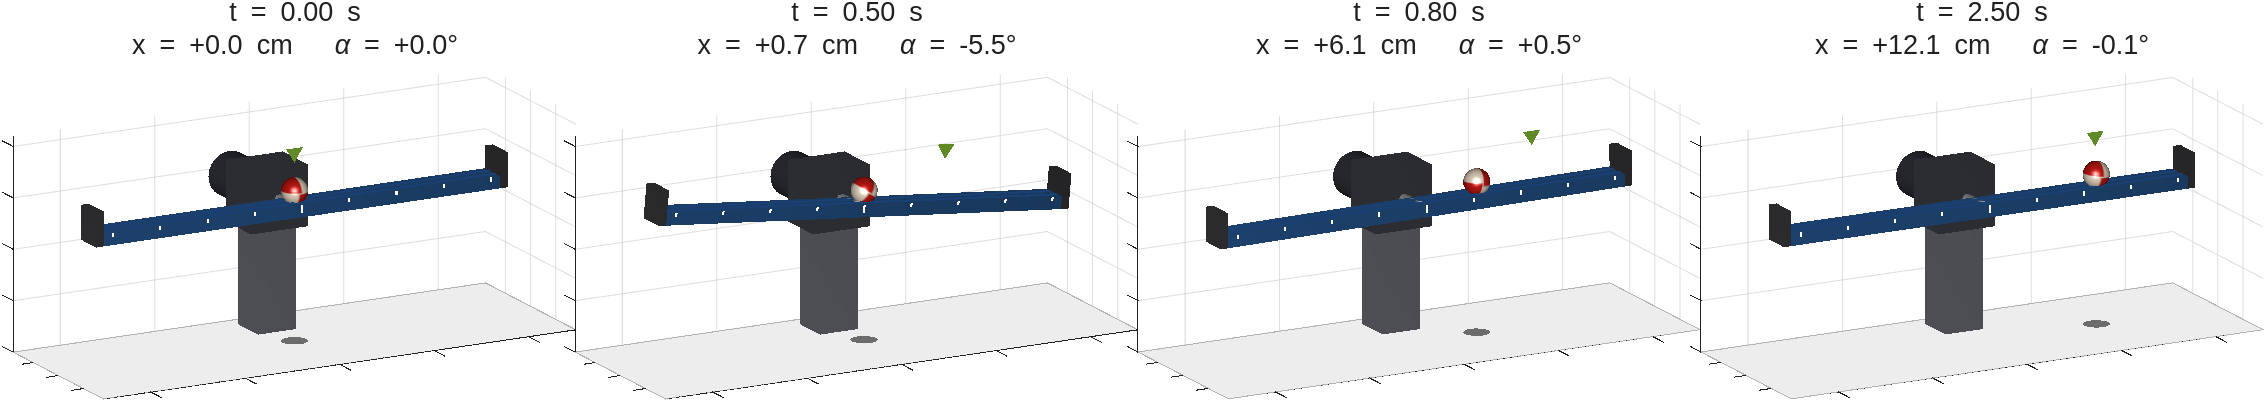
\includegraphics[width=\linewidth]{data/frames.png}
\caption{Fotogramas de la animación 3D (\code{bb\_animate}) durante un escalón de la referencia a \SI{12}{cm}. La bola tiene dos colores para que se vea girar; el triángulo verde marca la referencia.}
\label{fig:frames}
\end{figure}

\chapter{Modelado dinámico}
\label{cap:modelo}

\section{Cinemática}

Tomamos como coordenadas generalizadas $\vect q=[x,\ \alpha]^\top$. La viga gira alrededor de su centro, y la bola, de masa $m$ y radio $r_b$, se desplaza a lo largo de ella. Despreciando la pequeña distancia entre el centro de la bola y el eje de giro, la posición del centro de la bola es
\begin{equation}
  \vect p = x\,(\cos\alpha,\ \sin\alpha), \qquad |\dot{\vect p}|^2 = \xd^2 + x^2\ald^2 .
\end{equation}
El segundo término es la velocidad de arrastre: aunque la bola no se mueva respecto a la viga, si la viga gira la bola describe un arco de radio $|x|$.

\paragraph{Rodadura sin deslizamiento.} La bola rueda sobre la viga, de modo que su velocidad angular \emph{relativa} a la viga es $\xd/r_b$. Su velocidad angular absoluta es la de la viga más la relativa:
\begin{equation}
  \omega_b = \ald - \frac{\xd}{r_b}.
\end{equation}
La bola es una esfera maciza con $J_b=\tfrac25 mr_b^2$ respecto a su centro.

\section{Energías}

Sea $J$ la inercia de la viga respecto al pivote, incluida la inercia del rotor del motor reflejada a través de la reductora. La energía cinética total es
\begin{equation}
  T = \tfrac12 J\ald^2 + \tfrac12 m\left(\xd^2 + x^2\ald^2\right) + \tfrac12 J_b\left(\ald - \frac{\xd}{r_b}\right)^2 .
\end{equation}
Agrupando términos con la \emph{masa efectiva de rodadura}
\begin{equation}
  m_b = m + \frac{J_b}{r_b^2} = \tfrac75 m,
  \label{eq:mb}
\end{equation}
queda
\begin{equation}
  \boxed{T = \tfrac12 m_b\xd^2 - \frac{J_b}{r_b}\,\xd\ald + \tfrac12\left(J + J_b + m x^2\right)\ald^2}
  \label{eq:T}
\end{equation}
La energía potencial, con origen en el pivote y $\alpha>0$ levantando el extremo $+x$, es $U = m g x\sin\alpha$. El peso propio de la viga no aporta par porque su centro de masas está en el pivote.

\section{Ecuaciones de Euler--Lagrange}

Las fuerzas generalizadas no conservativas son la fricción de rodadura de la bola $b_x\xd$, una perturbación $F_d$ sobre la bola a lo largo de la viga, el par del motor $\tau$ y la fricción de la reductora:
\begin{equation}
  Q_x = F_d - b_x\xd,\qquad
  Q_\alpha = \tau - D_b\ald - T_c\operatorname{sgn}\ald .
\end{equation}

\paragraph{Coordenada $x$.}
\begin{equation}
  m_b\xdd - \frac{J_b}{r_b}\aldd - m x\ald^2 + m g\sin\alpha = Q_x .
  \label{eq:el1}
\end{equation}

\paragraph{Coordenada $\alpha$.}
\begin{equation}
  -\frac{J_b}{r_b}\xdd + \left(J+J_b+mx^2\right)\aldd + 2m x\xd\ald + m g x\cos\alpha = Q_\alpha .
  \label{eq:el2}
\end{equation}

Cada término tiene una interpretación directa:
\begin{itemize}
  \item $m g\sin\alpha$: la componente del peso a lo largo de la viga. Es la que mueve la bola.
  \item $m x\ald^2$: fuerza centrífuga. Si la viga gira deprisa, la bola tiende a salir hacia los extremos.
  \item $m g x\cos\alpha$: el par que el peso de la bola ejerce sobre la viga. Si la bola está en $x>0$, tiende a bajar el extremo $+x$ ($\aldd<0$).
  \item $2m x\xd\ald$: término de Coriolis; al alejarse la bola del pivote aumenta la inercia de la viga, $mx^2$.
  \item $J_b/r_b$: acoplamiento por el giro de la bola. Es pequeño ($J_b/r_b=\SI{3.4e-4}{kg.m}$) pero se mantiene.
\end{itemize}

\section{Forma matricial}

\begin{equation}
  \underbrace{\begin{bmatrix} m_b & -J_b/r_b\\ -J_b/r_b & J+J_b+mx^2\end{bmatrix}}_{\vect M(x)}
  \begin{bmatrix}\xdd\\ \aldd\end{bmatrix}
  =
  \begin{bmatrix}
    m x\ald^2 - m g\sin\alpha - b_x\xd + F_d + F_{\text{tope}}\\
    \tau - D_b\ald - T_c\tanh(\ald/\omega_\epsilon) - 2m x\xd\ald - m g x\cos\alpha + T_{\text{tope}}
  \end{bmatrix}.
  \label{eq:nl}
\end{equation}
Esta es exactamente la ecuación que implementa \code{bb\_plant\_block.m}, que resuelve el sistema $2\times2$ en cada paso del integrador. La matriz de masas es definida positiva: $\det\vect M = m_b(J+mx^2) + mJ_b > 0$.

\paragraph{Topes.} La bola choca con dos topes en $x=\pm x_{\max}$, con $x_{\max}=L/2-r_b=\SI{19.7}{cm}$, y la viga con dos topes en $\alpha=\pm\alpha_{\max}=\pm20^\circ$. Ambos se modelan como muelles-amortiguadores rígidos que solo empujan, nunca tiran ($F_{\text{tope}}$, $T_{\text{tope}}$).

\section{Motor, reductora y amplificador}

El motor de corriente continua mueve la viga a través de una reductora de relación $K_g=70$. Despreciando la inductancia del inducido, el par en el eje de salida es
\begin{equation}
  \tau = \eta_g\eta_m K_g\frac{k_t}{R_m}\left(V - K_gk_m\ald\right) = k_v\left(V - K_gk_m\ald\right),
  \qquad k_v = \frac{\eta_g\eta_mK_gk_t}{R_m}=\SI{0.128}{N.m/V},
  \label{eq:motor}
\end{equation}
con $\eta_g$ y $\eta_m$ los rendimientos de la reductora y del motor. La fuerza contraelectromotriz, multiplicada por $K_g$ dos veces, se convierte en un amortiguamiento viscoso considerable sobre la viga:
\begin{equation}
  b_{\text{eq}} = k_vK_gk_m + D_b = \SI{0.0690}{} + \SI{0.0010}{} = \SI{0.0700}{N.m.s/rad}.
\end{equation}
Del mismo modo, la inercia del rotor aparece multiplicada por $K_g^2$: $\eta_gK_g^2J_m=\SI{1.72e-3}{kg.m^2}$, un tercio de la inercia de la propia viga ($\SI{5.15e-3}{kg.m^2}$). El amplificador satura la tensión en $\pm\SI{10}{V}$, de modo que el par máximo es $k_vV_{\max}=\SI{1.28}{N.m}$. El par máximo que puede ejercer la bola sobre la viga es $mgx_{\max}=\SI{0.13}{N.m}$, es decir, mantener la viga horizontal con la bola en un extremo cuesta \SI{1.0}{V}.

\begin{ejemplo}{Matriz de masas y magnitudes derivadas}
Con los valores de la tabla~\ref{tab:param}: $J_b=\SI{4.32e-6}{kg.m^2}$, $m_b=\SI{0.0938}{kg}$ y $J=\SI{6.86e-3}{kg.m^2}$. Con la bola en el pivote:
\[
\vect M(0)=\begin{bmatrix}0{,}0938 & -3{,}40\cdot10^{-4}\\ -3{,}40\cdot10^{-4} & 6{,}87\cdot10^{-3}\end{bmatrix}.
\]
El acoplamiento fuera de la diagonal es dos órdenes de magnitud menor que los términos diagonales: el giro de la bola apenas afecta a la viga. Lo que sí importa es el factor $m/m_b=5/7$: una bola que rueda acelera un 29\,\% menos que una que deslizara sin fricción.
\end{ejemplo}

\section{Fricción}

\begin{itemize}
  \item \textbf{Viga}: viscosa $D_b\ald$ más Coulomb $T_c\tanh(\ald/\omega_\epsilon)$ en la reductora, con $T_c=\SI{0.01}{N.m}$. La tangente hiperbólica suaviza el signo para que el integrador de paso fijo no oscile alrededor de $\ald=0$.
  \item \textbf{Bola}: fricción de rodadura viscosa, $b_x\xd$, muy pequeña.
\end{itemize}
La fricción de Coulomb de la reductora equivale a \SI{0.08}{V}: es pequeña frente a las tensiones de trabajo, pero produce pequeños errores de posicionado de la viga que el lazo de la bola debe corregir.

\section{Parámetros por defecto}

\begin{table}[H]
\centering\small
\begin{tabular}{@{}llll@{}}
\toprule
Parámetro & Símbolo & Valor & Campo en \code{P}\\
\midrule
Masa de la bola & $m$ & \SI{0.067}{kg} & \code{m}\\
Radio de la bola & $r_b$ & \SI{12.7}{mm} & \code{rb}\\
Fricción de rodadura & $b_x$ & \SI{2e-3}{N.s/m} & \code{bx}\\
Longitud de la viga & $L$ & \SI{0.42}{m} & \code{L}\\
Masa de la viga & $m_{\text{viga}}$ & \SI{0.35}{kg} & \code{mbeam}\\
Fricción viscosa de la viga & $D_b$ & \SI{1e-3}{N.m.s/rad} & \code{Db}\\
Fricción de Coulomb de la viga & $T_c$ & \SI{0.01}{N.m} & \code{Tc}\\
Resistencia del motor & $R_m$ & \SI{2.6}{\ohm} & \code{Rm}\\
Constantes del motor & $k_t$, $k_m$ & \SI{7.68e-3}{N.m/A}, \SI{7.68e-3}{V.s/rad} & \code{kt}, \code{km}\\
Inercia del rotor & $J_m$ & \SI{3.9e-7}{kg.m^2} & \code{Jm}\\
Reductora y rendimientos & $K_g$, $\eta_g$, $\eta_m$ & 70; 0,9; 0,69 & \code{Kg}, \code{eta\_g}, \code{eta\_m}\\
Saturación del amplificador & $V_{\max}$ & \SI{10}{V} & \code{Vmax}\\
\bottomrule
\end{tabular}
\caption{Parámetros físicos por defecto (\code{bb\_params.m}). Son valores típicos de una maqueta de laboratorio de sobremesa. La tabla completa está en el apéndice~\ref{cap:parametros}.}
\label{tab:param}
\end{table}

\begin{aviso}
$J_b$, $m_b$, $J$, $x_{\max}$, $k_v$ y $b_{\text{eq}}$ son \emph{derivados}: los recalcula \code{bb\_derived} (llamada desde \code{bb\_design}) a partir de las masas, longitudes y constantes del motor. Si se cambia \code{m} o \code{L} con \code{setParam}, todo se actualiza. Con \code{setParamRaw} no se recalcula nada (sección~\ref{sec:robustez}).
\end{aviso}

\chapter{Análisis lineal}
\label{cap:analisis}

\section{Linealización}

Con la viga horizontal y la bola en reposo, \emph{cualquier} posición $x_0$ de la bola es un equilibrio, siempre que el motor compense el par que hace la bola sobre la viga:
\begin{equation}
  V_{\text{eq}}(x_0) = \frac{m g x_0}{k_v} .
  \label{eq:veq}
\end{equation}
Linealizamos alrededor de $x_0=0$, $\alpha=0$. Los términos centrífugo y de Coriolis son de segundo orden y desaparecen; $\sin\alpha\approx\alpha$ y $\cos\alpha\approx1$:
\begin{equation}
  \underbrace{\begin{bmatrix} m_b & -J_b/r_b\\ -J_b/r_b & J+J_b\end{bmatrix}}_{\vect M_0}
  \begin{bmatrix}\xdd\\ \aldd\end{bmatrix}
  =
  \begin{bmatrix} -m g\,\alpha - b_x\xd\\ k_vV - b_{\text{eq}}\ald - m g\,x\end{bmatrix}.
  \label{eq:lin}
\end{equation}
Despejando las aceleraciones y con $\vect s=[x,\ \xd,\ \alpha,\ \ald]^\top$ se obtiene $\dot{\vect s}=A\vect s+BV$, $\vect y=C\vect s$, con $C=\left[\begin{smallmatrix}1&0&0&0\\0&0&1&0\end{smallmatrix}\right]$. Es lo que calcula \code{bb\_linearize(P)}. La fricción de Coulomb se desprecia.

\begin{ejemplo}{Matrices numéricas (\code{bb\_linearize})}
\[
A=\begin{bmatrix}0&1&0&0\\ -0{,}347&-0{,}021&-7{,}008&-0{,}037\\ 0&0&0&1\\ -95{,}7&-0{,}001&-0{,}347&-10{,}20\end{bmatrix},\qquad
B=\begin{bmatrix}0\\ 0{,}068\\ 0\\ 18{,}70\end{bmatrix}.
\]
Los dos elementos dominantes cuentan casi toda la historia:
\begin{itemize}
  \item $A(2,3)=-7{,}008\approx-\tfrac57g$: inclinar la viga un radián acelera la bola a $\SI{7}{m/s^2}$ hacia el extremo bajo.
  \item $A(4,1)=-mg/J=-95{,}7$: la bola en $x>0$ hace caer el extremo $+x$ de la viga.
\end{itemize}
Los términos pequeños ($-0{,}347$, $0{,}068$, \ldots) vienen del acoplamiento por el giro de la bola, $J_b/r_b$.
\end{ejemplo}

\section{Polos en lazo abierto}

\begin{equation}
  \lambda_{\text{LA}} = \{-10{,}68,\quad +3{,}62,\quad -1{,}58\pm j3{,}85\}.
\end{equation}
Despreciando el acoplamiento por el giro de la bola y la fricción de rodadura, el polinomio característico tiene una forma muy instructiva:
\begin{equation}
  s^3\left(Js + b_{\text{eq}}\right) = mg\cdot\tfrac57 g
  \quad\Longrightarrow\quad
  \lambda\approx\{-10{,}74,\ +3{,}65,\ -1{,}55\pm j3{,}84\}.
  \label{eq:caract}
\end{equation}
El lado izquierdo es el de una viga sin bola ($s(Js+b_{\text{eq}})$, un integrador y el polo mecánico en $-b_{\text{eq}}/J=-10{,}2$) en serie con la bola como doble integrador ($s^2$). El lado derecho es el lazo que cierra el peso de la bola: la bola inclina la viga hacia su lado y la viga acelera la bola en el mismo sentido. Es una \textbf{realimentación positiva} que convierte los tres polos en el origen en un polo real inestable ($+3{,}62$, constante de tiempo de \SI{0.28}{s}) y un par complejo estable.

\begin{nota}
En la literatura es habitual estudiar la bola y viga con la viga posicionada por un servo ideal, $\ddot x=-\tfrac57g\alpha$. Ese modelo es un doble integrador puro y no tiene el polo en $+3{,}62$. Aquí la viga está movida directamente por el motor, y el peso de la bola importa: un par de \SI{0.13}{N.m} con la bola en el extremo frente a los \SI{1.28}{N.m} del motor saturado.
\end{nota}

\section{Funciones de transferencia}

\paragraph{Tensión a posición de la bola.}
\begin{equation}
  G_x(s)=\frac{X(s)}{V(s)} = \frac{0{,}068\,(s-43{,}9)(s+43{,}9)}{(s+10{,}68)(s-3{,}62)(s^2+3{,}16s+17{,}3)} .
\end{equation}
Para frecuencias bajas, $G_x(s)\approx-130/[(s+10{,}68)(s-3{,}62)(s^2+3{,}16s+17{,}3)]$: \textbf{relativo de grado 4}, con un desfase que crece deprisa. Los ceros en $\pm43{,}9$ son consecuencia del giro de la bola: una aceleración brusca de la viga empuja la bola directamente a través de su inercia de rotación ($-J_b/r_b\,\aldd$ en~\eqref{eq:el1}). Están lejos de la banda de trabajo y apenas influyen, pero formalmente el sistema es de fase no mínima.

\paragraph{Tensión a ángulo de la viga.}
\begin{equation}
  G_\alpha(s)=\frac{A(s)}{V(s)} = \frac{18{,}70\,s\,(s+0{,}021)}{(s+10{,}68)(s-3{,}62)(s^2+3{,}16s+17{,}3)} .
\end{equation}
El cero en el origen tiene una lectura física clara: en un equilibrio la bola está quieta, así que la viga debe estar horizontal; una tensión constante no inclina la viga en régimen permanente, sino que \emph{desplaza la posición de equilibrio de la bola}, según~\eqref{eq:veq}.

\begin{figure}[H]
\centering
\begin{tikzpicture}
\begin{groupplot}[group style={group size=1 by 2,vertical sep=0.4cm,xticklabels at=edge bottom},
  manual,height=4.3cm,xmode=log,xmin=0.1,xmax=100]
\nextgroupplot[ylabel={Magnitud [dB]},legend pos=north east]
\addplot[c1] table[x=f,y=mag]{data/bode_x.dat};
\addplot[c2] table[x=f,y=mag]{data/bode_al.dat};
\legend{$X/V$ [m/V],$A/V$ [rad/V]}
\nextgroupplot[ylabel={Fase [$^\circ$]},xlabel={$f$ [Hz]}]
\addplot[c1] table[x=f,y=ph]{data/bode_x.dat};
\addplot[c2] table[x=f,y=ph]{data/bode_al.dat};
\end{groupplot}
\end{tikzpicture}
\caption{Diagrama de Bode del modelo lineal. Entre \SI{2}{Hz} y \SI{7}{Hz}, $X/V$ cae \SI{36}{dB}: la bola apenas responde a tensiones rápidas.}
\label{fig:bode}
\end{figure}

\section{Controlabilidad y observabilidad}

\begin{itemize}
  \item \textbf{Controlabilidad}: la matriz $\mathcal C=[B,\ AB,\ A^2B,\ A^3B]$ tiene rango 4, aunque con un número de condición alto ($\approx10^4$): la bola se controla \emph{a través} de la viga, con tres integraciones de por medio.
  \item \textbf{Observabilidad desde $x$}: rango 4.
  \item \textbf{Observabilidad desde $\alpha$}: también rango 4, a diferencia del péndulo rotacional. El par que hace el peso de la bola deja su huella en el movimiento de la viga, así que en teoría se podría reconstruir $x$ midiendo solo $\alpha$. En la práctica la estimación sería muy sensible a errores en $m$ y en la fricción, y por eso se mide $x$ directamente.
\end{itemize}

\section{Lectura en cascada}

La estructura de~\eqref{eq:lin} sugiere dividir el sistema en dos:
\begin{equation}
  \underbrace{V\ \xrightarrow{\ \text{motor + viga}\ }\ \alpha}_{\text{rápido: } \tau\approx J/b_{\text{eq}}=\SI{0.1}{s}}
  \qquad\qquad
  \underbrace{\alpha\ \xrightarrow{\ -\frac57 g/s^2\ }\ x}_{\text{lento: doble integrador}}
\end{equation}
Si un lazo interno hace que $\alpha$ siga a una referencia $\alpha_r$ mucho más deprisa de lo que se mueve la bola, el lazo externo ve una planta $X/A_r\approx-\tfrac57g/s^2$ y se puede diseñar con un PD o un PID clásico. Es la idea del controlador en cascada (sección~\ref{sec:cascada}). El precio es que el lazo interno tiene que ser rígido frente al par $mgx$ de la bola, o se necesita compensarlo (sección~\ref{sec:ff}).

\chapter{Sensores y muestreo}
\label{cap:sensores}

\section{Posición de la bola}

La bola de acero hace contacto con una pista resistiva a lo largo de la viga y funciona como el cursor de un potenciómetro. La tensión se lee con un convertidor de 12 bits que cubre toda la longitud de la viga:
\begin{equation}
  q_x = \frac{L}{4096} = \SI{0.103}{mm}.
\end{equation}

\section{Ángulo de la viga}

Un encoder de 1024 líneas en cuadratura, montado en el eje de salida de la reductora, da 4096 cuentas por vuelta:
\begin{equation}
  q_\alpha = \frac{2\pi}{4096} = \SI{1.53}{mrad} = 0{,}088^\circ .
\end{equation}
En el modelo, cada medida pasa por un bloque \emph{Quantizer}, un ruido gaussiano opcional (\code{noise\_on}, con $\sigma_x=\SI{1}{mm}$ y $\sigma_\alpha=\SI{1}{mrad}$) y un muestreo a $T_s=\SI{2}{ms}$.

\section{Elección del periodo de muestreo}

El polo más rápido del lazo cerrado con el LQR por defecto está en \SI{16.6}{rad/s}, y el del lazo interno de la cascada en unos \SI{27}{rad/s}. Muestreando 20--40 veces más rápido bastarían \SIrange{90}{170}{Hz}. Los \SI{500}{Hz} elegidos, los mismos que en los péndulos, dan un margen amplio y permiten que el lazo interno de la viga sea rígido.

\section{Estimación de velocidades}

Las velocidades $\xd$ y $\ald$ se estiman con una derivada filtrada de primer orden, discretizada de forma exacta, igual que en los péndulos:
\begin{equation}
  v_k = a\,v_{k-1} + (1-a)\,\frac{y_k-y_{k-1}}{T_s},\qquad a = e^{-T_s/\tau}.
\end{equation}
Las dos constantes de tiempo son distintas porque las dos señales lo son:
\begin{itemize}
  \item \textbf{Viga}: $\tau_v=\SI{5}{ms}$ (derivada pura hasta \SI{32}{Hz}). El lazo interno es rápido y necesita poco retraso.
  \item \textbf{Bola}: $\tau_x=\SI{20}{ms}$ (\SI{8}{Hz}). Un salto de una cuenta en un periodo de muestreo se interpreta como una velocidad de $q_x/T_s=\SI{5.1}{cm/s}$, demasiado para una bola que se mueve a unos pocos cm/s cerca del equilibrio. La bola es lenta y admite más filtrado.
\end{itemize}

\begin{figure}[H]
\centering
\begin{tikzpicture}
\begin{axis}[manual,height=5cm,xmin=0,xmax=0.5,xlabel={$t$ [s]},ylabel={$\xd$ [m/s]},legend pos=south west,legend columns=3]
\addplot[gray!60,const plot,line width=0.5pt] table[x=t,y=raw]{data/velest.dat};
\addplot[c2] table[x=t,y=filt]{data/velest.dat};
\addplot[black,dashed] table[x=t,y=true]{data/velest.dat};
\legend{diferencia directa,filtrada ($\tau_x=\SI{20}{ms}$),real}
\end{axis}
\end{tikzpicture}
\caption{Estimación de $\xd$ a partir de $x=0{,}1\sin(2\pi t)$ cuantizada a \SI{0.103}{mm}. La diferencia directa salta entre múltiplos de \SI{5.1}{cm/s}; la filtrada es suave, pero llega con unos \SI{20}{ms} de retraso.}
\label{fig:velest}
\end{figure}

\section{Ruido y rizado de la tensión}

Con solo la cuantización, la tensión en equilibrio (LQR) tiene un rizado de \SI{0.10}{V} eficaces. Al activar el ruido de medida sube a \SI{0.85}{V} eficaces: el ruido de \SI{1}{mm} en $x$ es diez veces la resolución, y las ganancias del LQR sobre $x$ y $\xd$ ($K_x=\SI{-43.5}{V/m}$, $K_{\dot x}=\SI{-15.7}{V.s/m}$) lo amplifican. A pesar de ello, la bola real solo se mueve \SI{0.19}{mm} eficaces, porque la viga y la bola filtran mecánicamente esa tensión rápida. Es un buen punto de partida para la práctica del observador (capítulo~\ref{cap:practicas}).

\chapter{Diseño de controladores}
\label{cap:control}

El controlador discreto (\code{bb\_controller\_block.m}) ofrece cuatro modos, seleccionables en vivo:

\begin{table}[H]
\centering\small
\begin{tabular}{@{}cll@{}}
\toprule
Modo & Nombre & Ley de control\\
\midrule
0 & \code{open} & $V=u_{\text{manual}}+u_{\text{ext}}$ (lazo abierto, identificación)\\
1 & \code{beam} & PD del ángulo de la viga a $\alpha_{\text{manual}}$; la bola queda libre\\
2 & \code{cascade} & PID de la bola $\to\alpha_r\to$ PD de la viga, más prealimentación del peso\\
3 & \code{lqr} & $V=-K[x-r,\ \xd,\ \alpha,\ \ald,\ \textstyle\int(x-r)]^\top+V_{\text{eq}}(r)$\\
\bottomrule
\end{tabular}
\caption{Modos de control.}
\end{table}

Al cambiar de modo, o al deshabilitar el control, el integrador se pone a cero.

\section{El lazo interno: servo del ángulo de la viga}
\label{sec:interno}

El modo \code{beam} y la cascada comparten un PD sobre el ángulo de la viga:
\begin{equation}
  V = K_{pa}\left(\alpha_r-\alpha\right) - K_{da}\ald,\qquad K_{pa}=\SI{40}{V/rad},\ K_{da}=\SI{1.5}{V.s/rad}.
\end{equation}
Con la bola fuera ($m\to0$) el lazo cerrado de la viga es de segundo orden: $Js^2+(b_{\text{eq}}+k_vK_{da})s+k_vK_{pa}=0$, con $\omega_n=\SI{27}{rad/s}$ y $\zeta=0{,}70$. La figura~\ref{fig:interno} lo comprueba sobre el modelo no lineal con una bola de masa despreciable: un escalón de $5^\circ$ llega al 95\,\% en \SI{0.11}{s} con un 0,8\,\% de sobreoscilación. El error final ($4{,}97^\circ$) es la fricción de Coulomb: un PD sin integral no la elimina.

\begin{figure}[H]
\centering
\begin{tikzpicture}
\begin{axis}[manual,height=4.2cm,xmin=0,xmax=0.6,xlabel={$t$ [s]},ylabel={$\alpha$ [$^\circ$]},legend pos=south east]
\addplot[c1] table[x=t,y=al]{data/inner_step.dat};
\addplot[black,dashed] table[x=t,y=alr]{data/inner_step.dat};
\legend{$\alpha$,$\alpha_r$}
\end{axis}
\end{tikzpicture}
\caption{Lazo interno: escalón de $5^\circ$ en el modo \code{beam} con la bola retirada (\code{setParam('m', 1e-5)}).}
\label{fig:interno}
\end{figure}

Con la bola puesta, el mismo PD deja la bola libre: es la forma de \textbf{ver la inestabilidad en lazo abierto}. Con la viga a $-2^\circ$ la bola llega al tope en \SI{1.28}{s} (con la viga fija y rígida serían $\sqrt{2x_{\max}/(\tfrac57g\sin2^\circ)}=\SI{1.27}{s}$). Mientras rueda, su peso inclina la viga hasta $-3{,}0^\circ$: un PD de rigidez finita no puede mantener el ángulo frente a una carga que crece con $x$.

\section{Control en cascada}
\label{sec:cascada}

\subsection{Lazo externo}
Con el lazo interno mucho más rápido que la bola, la bola ve $\ddot x\approx-\tfrac57g\,\alpha_r$. El lazo externo es un PID que calcula la inclinación necesaria:
\begin{equation}
  \alpha_r = \operatorname{sat}_{\pm\alpha_{r,\max}}\!\left(K_{px}(x-r) + K_{dx}\xd + K_{ix}\!\int(x-r)\,\dd t\right),
\end{equation}
con $K_{px}=\SI{1.3}{rad/m}$, $K_{dx}=\SI{0.8}{rad.s/m}$, $K_{ix}=\SI{0.1}{rad/(m.s)}$ y $\alpha_{r,\max}=0{,}25$~rad ($14^\circ$). Los signos son los intuitivos: si la bola se pasa de la referencia ($x>r$), se levanta el extremo $+x$ ($\alpha_r>0$) para que vuelva. Con un lazo interno ideal y sin integral, el lazo externo es
\begin{equation}
  s^2 + \tfrac57gK_{dx}\,s + \tfrac57gK_{px} = s^2 + 5{,}6\,s + 9{,}1 = 0
  \quad\Rightarrow\quad \omega_n=\SI{3.0}{rad/s},\ \zeta=0{,}93,
\end{equation}
diez veces más lento que el lazo interno: la separación de escalas que justifica la cascada. Sobre el modelo lineal completo, la cascada PD (sin integral) equivale a una realimentación de estado con polos $-14{,}3\pm j17{,}8$, $-5{,}13$ y $-2{,}30$.

\subsection{Prealimentación del peso de la bola}
\label{sec:ff}

En equilibrio con la bola en $x$, el motor tiene que hacer un par $mgx$ (ecuación~\eqref{eq:veq}). Con un PD en el lazo interno, ese par solo aparece si hay un error $\alpha_r-\alpha=V_{\text{eq}}/K_{pa}$, y ese $\alpha_r$ solo aparece si la bola está desplazada de la referencia. Con $r=\SI{10}{cm}$:
\[
V_{\text{eq}}=\SI{0.57}{V}\ \Rightarrow\ \alpha_r=\frac{0{,}57}{40}=\SI{0.014}{rad}\ \Rightarrow\ x-r=\frac{0{,}014}{1{,}3}=\SI{1.1}{cm}.
\]
Es exactamente el error que se mide sin prealimentación ni integral (figura~\ref{fig:ff}). La solución es sumar a la tensión el término $m g x/k_v$ calculado con la $x$ medida (\code{ff\_on = 1}). Con ella la bola llega a $\SI{9.99}{cm}$ sin necesidad de integral; el integrador queda para corregir errores de modelo.

\begin{figure}[H]
\centering
\begin{tikzpicture}
\begin{axis}[manual,height=4.6cm,xmin=0,xmax=6,xlabel={$t$ [s]},ylabel={$x$ [cm]},legend pos=south east]
\addplot[c1] table[x=t,y=x]{data/ff_1.dat};
\addplot[c2] table[x=t,y=x]{data/ff_0.dat};
\addplot[c4] table[x=t,y=x]{data/lqr_noff.dat};
\addplot[black,dashed] table[x=t,y=r]{data/ff_1.dat};
\legend{cascada con prealim.,cascada sin prealim.,LQR sin prealim.,$r$}
\end{axis}
\end{tikzpicture}
\caption{Efecto de la prealimentación del peso (cascada sin integral, $K_{ix}=0$). Sin ella la bola se queda \SI{1.1}{cm} más allá de la referencia. El LQR sin prealimentación también se pasa \SI{1.2}{cm}, y su integrador tarda \SI{3.6}{s} en corregirlo.}
\label{fig:ff}
\end{figure}

\subsection{Antisaturación del integrador}
El integrador solo acumula cuando $|x-r|<e_{\text{int}}=\SI{2}{cm}$ (integración condicional) y además se recorta a $\pm I_{\max}$. Durante los movimientos grandes no integra, y no hay sobreoscilación por \emph{windup}.

\section{LQR con acción integral}
\label{sec:lqr}

\subsection{Planteamiento}
Se amplía el estado con la integral del error, $\xi=\int(x-r)\,\dd t$, y se minimiza
\begin{equation}
  J=\int_0^\infty\left(\tilde{\vect s}^\top Q\,\tilde{\vect s} + R\,V^2\right)\dd t,\qquad \tilde{\vect s}=[x-r,\ \xd,\ \alpha,\ \ald,\ \xi]^\top .
\end{equation}
\code{bb\_lqr} usa \code{lqr()} si existe la Control System Toolbox y, si no, el método del Hamiltoniano. A la ley $V=-K\tilde{\vect s}$ se le suma la tensión de equilibrio en la referencia, $V_{\text{eq}}(r)=mgr/k_v$, que es la prealimentación correspondiente.

\begin{ejemplo}{Ganancias por defecto}
Con $Q=\operatorname{diag}(1000;\ 50;\ 10;\ 0{,}5;\ 200)$ y $R=1$:
\[
K=\begin{bmatrix}-43{,}5 & -15{,}7 & 18{,}8 & 1{,}18 & -14{,}1\end{bmatrix},\qquad
\lambda_{\text{LC}}=\{-16{,}6,\ -4{,}90\pm j5{,}78,\ -4{,}37,\ -0{,}44\}.
\]
Unidades: V/m, V/(m/s), V/rad, V/(rad/s) y V/(m\,s). Un error de \SI{1}{cm} pide \SI{0.43}{V}; una inclinación de $1^\circ$, \SI{-0.33}{V}. El cociente $K_x/K_\alpha=\SI{2.3}{rad/m}$ es la inclinación «pedida» por unidad de error, del orden del $K_{px}$ de la cascada.
\end{ejemplo}

El polo lento en $-0{,}44$ es el del integrador: con $Q_\xi=200$ el LQR lo deja lento a propósito para que no sobreoscile. Como el integrador solo actúa cerca de la referencia, ese polo no frena los movimientos grandes, pero sí se nota en la recuperación tras una perturbación (figura~\ref{fig:tap}).

\begin{figure}[H]
\centering
\begin{tikzpicture}
\begin{groupplot}[group style={group size=1 by 3,vertical sep=0.35cm,xticklabels at=edge bottom},
  manual,height=3.5cm,xmin=0,xmax=3]
\nextgroupplot[ylabel={$x$ [cm]}]
\addplot[c1] table[x=t,y=x]{data/lqr_ic.dat};
\nextgroupplot[ylabel={$\alpha$ [$^\circ$]}]
\addplot[c2] table[x=t,y=al]{data/lqr_ic.dat};
\nextgroupplot[ylabel={$V$ [V]},xlabel={$t$ [s]}]
\addplot[c4] table[x=t,y=V]{data/lqr_ic.dat};
\end{groupplot}
\end{tikzpicture}
\caption{LQR desde $x_0=\SI{10}{cm}$. La viga se inclina hasta $9{,}6^\circ$ para lanzar la bola hacia el centro y después hasta $-5{,}9^\circ$ para frenarla. La bola queda a menos de \SI{5}{mm} del centro en \SI{0.68}{s}, con \SI{2.6}{mm} de sobreoscilación. Pico de tensión: \SI{4.4}{V}.}
\label{fig:lqric}
\end{figure}

\section{Comparación: escalón de referencia}

\begin{figure}[H]
\centering
\begin{tikzpicture}
\begin{groupplot}[group style={group size=1 by 3,vertical sep=0.35cm,xticklabels at=edge bottom},
  manual,height=3.5cm,xmin=0,xmax=4]
\nextgroupplot[ylabel={$x$ [cm]},legend pos=south east]
\addplot[c1] table[x=t,y=x]{data/lqr_step.dat};
\addplot[c2] table[x=t,y=x]{data/cascade_step.dat};
\addplot[black,dashed] table[x=t,y=r]{data/lqr_step.dat};
\legend{LQR,cascada,$r$ (limitada)}
\nextgroupplot[ylabel={$\alpha$ [$^\circ$]}]
\addplot[c1] table[x=t,y=al]{data/lqr_step.dat};
\addplot[c2] table[x=t,y=al]{data/cascade_step.dat};
\nextgroupplot[ylabel={$V$ [V]},xlabel={$t$ [s]}]
\addplot[c1] table[x=t,y=V]{data/lqr_step.dat};
\addplot[c2] table[x=t,y=V]{data/cascade_step.dat};
\end{groupplot}
\end{tikzpicture}
\caption{Escalón de \SI{10}{cm} en $t=\SI{1}{s}$, suavizado por el limitador de pendiente por defecto (\SI{0.3}{m/s}).}
\label{fig:step}
\end{figure}

\begin{table}[H]
\centering\small
\begin{tabular}{@{}lcccc@{}}
\toprule
Ensayo (escalón de \SI{10}{cm}) & Asentamiento a \SI{5}{mm} & Sobreoscilación & $V_{\max}$ & $\max|\alpha|$\\
\midrule
LQR, con limitador & \SI{0.85}{s} & 2,6\,\% & \SI{1.0}{V} & $5{,}9^\circ$\\
LQR, sin limitador & \SI{0.64}{s} & 2,5\,\% & \SI{3.8}{V} & $9{,}1^\circ$\\
Cascada, con limitador & \SI{1.67}{s} & 0,7\,\% & \SI{1.1}{V} & $3{,}5^\circ$\\
Cascada, sin limitador & \SI{1.50}{s} & 0,8\,\% & \SI{5.2}{V} & $6{,}9^\circ$\\
\bottomrule
\end{tabular}
\caption{Escalón de referencia: LQR frente a cascada.}
\label{tab:step}
\end{table}

El LQR es el doble de rápido con las ganancias por defecto, porque usa a la vez toda la información del estado; la cascada sacrifica velocidad a cambio de un diseño que se entiende y se ajusta lazo a lazo. Ninguno de los dos está cerca de saturar: la limitación real es el ángulo de la viga, no la tensión.

\subsection{Seguimiento de una senoide}
Con una referencia de $\pm\SI{10}{cm}$:

\begin{table}[H]
\centering\small
\begin{tabular}{@{}lcccc@{}}
\toprule
& \multicolumn{2}{c}{LQR} & \multicolumn{2}{c}{Cascada}\\
\cmidrule(lr){2-3}\cmidrule(lr){4-5}
Frecuencia & Ganancia & Retraso & Ganancia & Retraso\\
\midrule
\SI{0.1}{Hz} & 1,01 & $14^\circ$ & 0,94 & $23^\circ$\\
\SI{0.25}{Hz} & 0,96 & $35^\circ$ & 0,83 & $51^\circ$\\
\SI{0.5}{Hz} & 0,88 & $69^\circ$ & 0,58 & $88^\circ$\\
\bottomrule
\end{tabular}
\caption{Seguimiento de una referencia senoidal de $\pm\SI{10}{cm}$.}
\label{tab:sine}
\end{table}

El retraso del LQR crece casi linealmente con la frecuencia (unos \SI{0.38}{s} de retraso equivalente): se comporta como un filtro de fase casi lineal hasta \SI{0.5}{Hz}. La cascada tiene claramente menos ancho de banda: a \SI{0.5}{Hz} solo recorre el 58\,\% de la amplitud.

\subsection{Rechazo de perturbaciones}

\begin{figure}[H]
\centering
\begin{tikzpicture}
\begin{axis}[manual,height=4.4cm,xmin=0.5,xmax=4,xlabel={$t$ [s]},ylabel={$x$ [cm]},legend pos=north east]
\addplot[c1] table[x=t,y=x]{data/lqr_tap.dat};
\addplot[c2] table[x=t,y=x]{data/cascade_tap.dat};
\legend{LQR,cascada}
\end{axis}
\end{tikzpicture}
\caption{Golpecito de \SI{0.2}{N} durante \SI{50}{ms} sobre la bola en $t=\SI{1}{s}$. El LQR la desplaza \SI{1.93}{cm} y tarda \SI{2.2}{s} en volver a menos de \SI{2}{mm}; la cascada, \SI{1.69}{cm} y \SI{1.2}{s}.}
\label{fig:tap}
\end{figure}

Aquí la cascada gana. El golpe deja la bola dentro de la banda de integración, y el integrador del LQR, con su polo lento en $-0{,}44$, alarga la cola de la respuesta. Subir $Q_\xi$ acelera la recuperación a costa de más sobreoscilación en los escalones (práctica~\ref{pr:lqr}).

\subsection{Elección de los pesos}

\begin{figure}[H]
\centering
\begin{tikzpicture}
\begin{groupplot}[group style={group size=2 by 1,horizontal sep=1.6cm},
  manual,width=0.5\linewidth,height=5cm,xmin=0,xmax=3]
\nextgroupplot[ylabel={$x$ [cm]},xlabel={$t$ [s]},legend pos=north east,title={Barrido de $Q_x$ ($R=1$)}]
\addplot[c6] table[x=t,y=x]{data/qsweep_200.dat};
\addplot[c1] table[x=t,y=x]{data/qsweep_1000.dat};
\addplot[c4] table[x=t,y=x]{data/qsweep_5000.dat};
\legend{$200$,$1000$,$5000$}
\nextgroupplot[ylabel={$V$ [V]},xlabel={$t$ [s]},legend pos=north east,title={Barrido de $R$}]
\addplot[c2] table[x=t,y=V]{data/rsweep_0.1.dat};
\addplot[c1] table[x=t,y=V]{data/lqr_ic.dat};
\addplot[c5] table[x=t,y=V]{data/rsweep_10.dat};
\legend{$0{,}1$,$1$,$10$}
\end{groupplot}
\end{tikzpicture}
\caption{Efecto de los pesos del LQR (ensayo desde $x_0=\SI{10}{cm}$).}
\label{fig:pesos}
\end{figure}

\begin{table}[H]
\centering\small
\begin{tabular}{@{}lcccc@{}}
\toprule
Diseño & $K$ (sin $K_\xi$) & Asentamiento & $V_{\max}$ [V] & $\max|\alpha|$ [$^\circ$]\\
\midrule
$Q_x=200$ & $[-29{,}2\ \ -12{,}5\ \ 16{,}5\ \ 1{,}10]$ & \SI{1.24}{s} & 2,9 & 6,7\\
$Q_x=1000$ (defecto) & $[-43{,}5\ \ -15{,}7\ \ 18{,}8\ \ 1{,}18]$ & \SI{0.68}{s} & 4,4 & 9,6\\
$Q_x=5000$ & $[-80{,}6\ \ -23{,}5\ \ 23{,}7\ \ 1{,}36]$ & \SI{0.52}{s} & 8,1 & 16,1\\
$R=0{,}1$ & $[-124\ \ -44{,}5\ \ 45{,}3\ \ 2{,}79]$ & \SI{0.74}{s} & 10 (satura) & --\\
$R=10$ & $[-18{,}7\ \ -6{,}36\ \ 9{,}59\ \ 0{,}65]$ & \SI{2.50}{s} & 1,9 & --\\
\bottomrule
\end{tabular}
\caption{Ganancias y prestaciones para distintos pesos.}
\end{table}

Dos observaciones. Con $Q_x=5000$ la viga llega a $16^\circ$, cerca de los topes de $20^\circ$: en este sistema, \textbf{el recurso limitado es la inclinación}, porque la aceleración de la bola es $\tfrac57g\sin\alpha$. Y con $R=0{,}1$ el diseño satura el amplificador y acaba siendo \emph{más lento} que el de $R=1$: el LQR supone que la tensión pedida se aplica, y cuando no es así su optimalidad desaparece.

\section{Robustez frente a la masa de la bola}
\label{sec:robustez}

Para probar la robustez hay que cambiar la planta \emph{sin} recalcular las ganancias:
\begin{lstlisting}
Knom = bb.P.K;
bb.setParam('m', 0.134);      % bola el doble de pesada (recalcula todo...)
bb.setParamRaw('K', Knom);    % ...pero se impone de nuevo la ganancia nominal
\end{lstlisting}
La prealimentación sí usa la masa nueva, como si se conociera el peso de la bola.

\begin{table}[H]
\centering\small
\begin{tabular}{@{}lcc@{}}
\toprule
Masa de la bola & LQR nominal & Cascada\\
\midrule
\SI{30}{g} & \SI{0.80}{s}, 2,6\,\% & \SI{1.68}{s}, 0,7\,\%\\
\SI{67}{g} (nominal) & \SI{0.85}{s}, 2,6\,\% & \SI{1.67}{s}, 0,7\,\%\\
\SI{134}{g} & \SI{1.23}{s}, 2,8\,\% & \SI{1.67}{s}, 0,7\,\%\\
\SI{268}{g} & \SI{1.78}{s}, 4,0\,\% & \SI{1.66}{s}, 0,7\,\%\\
\bottomrule
\end{tabular}
\caption{Escalón de \SI{10}{cm} (con limitador) para distintas masas de la bola: tiempo de asentamiento a \SI{5}{mm} y sobreoscilación.}
\label{tab:masa}
\end{table}

La cascada es prácticamente insensible a la masa, por una razón física: la aceleración de la bola, $\tfrac57g\sin\alpha$, \emph{no depende de $m$}. La masa solo entra a través del par sobre la viga, que el lazo interno rígido y la prealimentación absorben. El LQR, en cambio, está diseñado con el acoplamiento $mg/J$ del modelo nominal; con cuatro veces la masa sigue siendo estable, pero el doble de lento.

\chapter{Implementación en Simulink}
\label{cap:simulink}

\section{Generación del modelo por script}

El modelo \code{ballbeam\_sim.slx} no se dibuja a mano: lo genera \code{bb\_build\_model.m} mediante \code{add\_block} y \code{add\_line}, igual que en los experimentos anteriores. De esta forma el modelo es reproducible y se reconstruye en segundos tras cualquier cambio. El código de los bloques \emph{MATLAB Function} se lee de \code{bb\_plant\_block.m}, \code{bb\_controller\_block.m} y \code{bb\_ref\_block.m}, y se inserta mediante la API de Stateflow:

\begin{lstlisting}[caption={Inserción del código de un bloque \emph{MATLAB Function} y declaración de \code{P} como parámetro.}]
rt = sfroot;
ch = rt.find('-isa', 'Stateflow.EMChart', 'Path', blkPath);
ch.Script = fileread('bb_controller_block.m');
d = ch.find('-isa', 'Stateflow.Data', 'Name', 'P');
d.Scope = 'Parameter';         % P se lee del workspace (struct ajustable)
\end{lstlisting}

\begin{aviso}
Si se edita alguno de los archivos \code{*\_block.m}, hay que volver a ejecutar \code{bb\_build\_model}. Los cambios hechos directamente sobre el \code{.slx} se pierden al regenerarlo.
\end{aviso}

\section{Arquitectura}

\begin{figure}[H]
\centering
\resizebox{\linewidth}{!}{%
\begin{tikzpicture}[>=Latex,font=\small,
  ss/.style={draw,very thick,fill=#1,minimum width=2.2cm,minimum height=1.5cm,align=center,rounded corners=1pt},
  ss/.default=c1!10,
  cst/.style={draw,fill=yellow!25,minimum width=1.6cm,minimum height=0.6cm,font=\footnotesize\ttfamily},
  fw/.style={draw,fill=orange!20,minimum width=1.6cm,minimum height=0.6cm,font=\footnotesize\ttfamily},
  sm/.style={draw,circle,inner sep=1pt}]
\node[cst] (clk) at (0,2.2) {Clock};
\node[cst] (cref) at (0,1.4) {cmd\_ref};
\node[fw] (rext) at (0,0.6) {ref\_ext};
\node[ss=gray!12] (ref) at (2.8,1.4) {Reference};
\node[cst] (cctrl) at (2.8,-1.0) {cmd\_ctrl};
\node[ss=c4!12] (ctl) at (5.6,0.4) {Controller};
\node[sm] (sf) at (7.6,0.6) {$+$};
\node[fw] (uext) at (7.6,1.7) {u\_ext};
\node[ss=c2!12] (act) at (9.6,0.6) {Amplifier};
\node[cst] (cd) at (11.4,2.3) {cmd\_dist};
\node[fw] (dext) at (12.9,2.3) {d\_ext};
\node[sm] (sd) at (12.2,1.4) {$+$};
\node[ss=c5!14] (pl) at (12.2,0.2) {Plant};
\node[ss=yellow!18] (sen) at (12.2,-2.0) {Sensors};
\node[draw,fill=gray!20,minimum height=4cm,minimum width=0.15cm] (mux) at (14.8,-0.4) {};
\node[draw,fill=c3!25,minimum width=1.5cm,minimum height=0.7cm,font=\footnotesize\ttfamily] (tel) at (16.4,-0.4) {telemetry};
\node[draw,fill=gray!10,minimum width=1.3cm,font=\footnotesize] (tw) at (18.4,0.3) {out.tel};
\node[draw,fill=gray!10,minimum width=1.3cm,font=\footnotesize] (sc) at (18.4,-1.1) {Scope};
\draw[->] (clk) -| ($(ref.west)+(-0.5,0.5)$) -- ($(ref.west)+(0,0.5)$);
\draw[->] (cref) -- (ref);
\draw[->] (rext) -| ($(ref.west)+(-0.5,-0.5)$) -- ($(ref.west)+(0,-0.5)$);
\draw[->] (ref.east) -- node[above]{$r$} ++(0.5,0) |- ($(ctl.west)+(0,0.3)$);
\draw[->] (cctrl) -| ($(ctl.west)+(-0.4,-0.45)$) -- ($(ctl.west)+(0,-0.45)$);
\draw[->] ($(ctl.east)+(0,0.2)$) -- node[above]{$V_c$} (sf);
\draw[->] (uext) -- (sf);
\draw[->] (sf) -- node[above]{$V_{\text{cmd}}$} (act);
\draw[->] (act) -- node[above]{$V$} ($(pl.west)+(0,0.4)$);
\draw[->] (cd) -| (sd); \draw[->] (dext) -| (sd);
\draw[->] (sd) -- node[right]{$F_d$} (pl);
\draw[->] (pl.east) -- node[above]{$\vect s$} ++(0.6,0) coordinate (b1) |- (sen.east);
\draw[->] (sen.west) -- ++(-1.5,0) -| node[pos=0.3,below]{$\vect y_m$} ($(ctl.south)+(-0.4,0)$);
\draw[->] (b1) -- ($(mux.west)+(0,0.6)$);
\draw[->,densely dotted] ($(ctl.east)+(0,-0.4)$) -- node[below,font=\footnotesize]{info} ++(0.7,0) |- (14.3,-3.2) |- ($(mux.west)+(0,-1.9)$);
\draw[->,densely dotted] (sen.east) ++(0,-0.3) -- ($(mux.west)+(0,-1.2)$);
\draw[->] (mux) -- (tel);
\draw[->] (tel) -- ++(0.9,0) |- (tw); \draw[->] (tel) -- ++(0.9,0) |- (sc);
\node[font=\scriptsize,align=left,anchor=north west] at (0,-1.7) {\colorbox{yellow!25}{\strut} Constant: modificable en vivo\\ \colorbox{orange!20}{\strut} From Workspace: se lee al arrancar};
\end{tikzpicture}}
\caption{Nivel superior del modelo \code{ballbeam\_sim}. Los bloques amarillos son el «panel de mando» que modifican la clase \code{BallBeam} y la GUI.}
\label{fig:arquitectura}
\end{figure}

\section{Subsistemas}

\begin{table}[H]
\centering\small
\begin{tabularx}{\linewidth}{@{}lp{3.2cm}X@{}}
\toprule
Subsistema & Entradas $\to$ salidas & Contenido\\
\midrule
\code{Reference} & $t$, \code{cmd\_ref}, \code{ref\_ext} $\to r$ & \emph{MATLAB Function} \code{bb\_ref\_block}: constante, seno, cuadrada, triangular o externa. Le siguen un \emph{Rate Limiter} ($\pm$\code{P.ref\_rate}, \SI{0.3}{m/s}) y una \emph{Saturation} ($\pm$\code{P.x\_ref\_max}, $\pm\SI{15}{cm}$).\\
\code{Controller} & $\vect y_m$, $r$, \code{cmd\_ctrl} $\to V_c$, info & ZOH sobre $r$ y \emph{MATLAB Function} \code{bb\_controller\_block}, con estado persistente (velocidades estimadas e integrador). Se ejecuta a $T_s$.\\
\code{Amplifier} & $V_{\text{cmd}}\to V$ & \emph{Saturation} $\pm V_{\max}$. La fuerza contraelectromotriz se calcula dentro de la planta.\\
\code{Plant} & $V$, $F_d\to\vect s$ & \emph{MATLAB Function} \code{bb\_plant\_block} (modelo~\eqref{eq:nl}, motor~\eqref{eq:motor} y topes) más un \emph{Integrator} vectorial con condición inicial \code{P.x0}.\\
\code{Sensors} & $\vect s\to\vect y_m$ & Selección de $x$ y $\alpha$, ruido (\emph{Random Number}$\times\sigma\times$\code{noise\_on}), \emph{Quantizer} y ZOH a $T_s$.\\
\bottomrule
\end{tabularx}
\caption{Contenido de cada subsistema.}
\end{table}

\section{Configuración de la simulación}

\begin{itemize}
  \item \textbf{Solver}: ode4 (Runge--Kutta) de paso fijo, con $h=\SI{1}{ms}$. El paso fijo hace la simulación determinista y compatible con el \emph{pacing}. La dinámica más rápida del lazo cerrado está por debajo de \SI{20}{rad/s}, así que $\omega h\approx0{,}02$. Los topes son rígidos ($k=\SI{2000}{N/m}$ para la bola): con la masa efectiva de la bola su frecuencia propia es de unos \SI{146}{rad/s}, todavía bien resuelta con $h=\SI{1}{ms}$.
  \item \textbf{Multifrecuencia}: la planta es continua y el controlador y los sensores son discretos a $T_s=2h$. Simulink inserta automáticamente las transiciones de frecuencia.
  \item \textbf{Parámetros}: todos los bloques leen sus parámetros del \emph{struct} \code{P} del workspace base. Con \code{DefaultParameterBehavior = Tunable}, basta con cambiar \code{P} y ejecutar\\ \code{set\_param(mdl, 'SimulationCommand', 'update')}\\ para aplicar el cambio en caliente.
  \item \textbf{Tiempo real}: \code{EnablePacing = on} y \code{PacingRate = 1} hacen que la simulación avance al ritmo del reloj de pared. Lo activa \code{BallBeam.start()} y lo desactiva \code{BallBeam.run()}.
  \item \textbf{Retrollamadas del modelo}: \code{InitFcn} crea \code{P} y las señales externas si no existen, para poder pulsar \emph{Run} directamente en Simulink. \code{StartFcn} y \code{StopFcn} conectan y desconectan el \emph{listener} de telemetría.
\end{itemize}

\section{Telemetría}

El bloque \code{telemetry} (una ganancia unidad, no virtual) concentra 12 señales. Se guardan en \code{out.tel} y además se leen en vivo con \code{add\_exec\_event\_listener}.

\begin{table}[H]
\centering\small
\begin{tabular}{@{}clll@{\hspace{1.2cm}}clll@{}}
\toprule
\# & Campo & Señal & Ud. & \# & Campo & Señal & Ud.\\
\midrule
1 & \code{x} & posición de la bola & m & 7 & \code{Vcmd} & tensión pedida & V\\
2 & \code{xd} & velocidad de la bola & m/s & 8 & \code{Vact} & tensión aplicada & V\\
3 & \code{al} & ángulo de la viga & rad & 9 & \code{r} & referencia filtrada & m\\
4 & \code{ald} & vel. de la viga & rad/s & 10 & \code{mode} & modo activo & --\\
5 & \code{xm} & $x$ medida & m & 11 & \code{alr} & referencia de $\alpha$ (cascada) & rad\\
6 & \code{alm} & $\alpha$ medido & rad & 12 & \code{I} & integrador & m\,s\\
\bottomrule
\end{tabular}
\caption{Vector de telemetría (\code{BallBeam.TEL}).}
\label{tab:tel}
\end{table}

\chapter{Interfaces de usuario: código y GUI}
\label{cap:codigo}

\section{La clase \code{BallBeam}}

\code{BallBeam} encapsula todo el acceso al modelo y tiene la misma interfaz que \code{CartPole} y \code{RotaryPendulum} en los péndulos. Permite trabajar de dos maneras:
\begin{itemize}
  \item \textbf{Por lotes} (\code{run(T)}): simula $T$ segundos tan rápido como puede y devuelve un \emph{struct} con todas las señales. Es la forma adecuada para diseñar, hacer barridos y generar figuras.
  \item \textbf{En vivo} (\code{start}/\code{stop}): simula indefinidamente en tiempo real. Los comandos tienen efecto inmediato y la telemetría llega a las funciones registradas como \emph{callback}. La primera vez tarda unos segundos en compilar el modelo.
\end{itemize}
Ambos modos dan exactamente el mismo resultado: el solver es de paso fijo y el \emph{pacing} solo frena el reloj, no cambia la integración.

\begin{figure}[H]
\centering
\resizebox{\linewidth}{!}{%
\begin{tikzpicture}[>=Latex,font=\small,
  ll/.style={draw,thick,minimum width=2.6cm,minimum height=0.8cm,fill=#1,align=center},ll/.default=gray!10,
  lab/.style={above,font=\scriptsize,fill=white,inner sep=1pt}]
\def\xa{0}\def\xb{6.5}\def\xc{13}
\node[ll=c1!12] (u) at (\xa,0) {Usuario /\\script / GUI};
\node[ll=c4!12] (c) at (\xb,0) {\code{BallBeam}};
\node[ll=c5!12] (s) at (\xc,0) {Simulink\\\code{ballbeam\_sim}};
\foreach \n in {u,c,s} \draw[dashed,gray] (\n.south) -- ++(0,-8.4);
\draw[->] (\xa,-1.1) -- node[lab]{\code{setMode}, \code{setRef}, \code{setInitialState}} (\xb,-1.1);
\draw[->] (\xb,-1.8) -- node[lab]{\code{set\_param(cmd\_*)}, \code{assignin('base','P')}} (\xc,-1.8);
\draw[->] (\xa,-2.6) -- node[lab]{\code{start()}} (\xb,-2.6);
\draw[->] (\xb,-3.3) -- node[lab]{\code{SimulationCommand=start} (pacing 1x)} (\xc,-3.3);
\draw[->,c2] (\xc,-4.0) -- node[lab]{\code{StartFcn}: \emph{listener} sobre \code{telemetry}} (\xb,-4.0);
\draw[->,c2] (\xc,-4.7) -- node[lab]{\code{PostOutputs} (cada paso)} (\xb,-4.7);
\draw[->,c2] (\xb,-5.4) -- node[lab]{\code{callback(t,d)} hasta 30 Hz} (\xa,-5.4);
\draw[->] (\xa,-6.2) -- node[lab]{\code{push(F,dur)}, \code{setRef(...)}, \code{setParam(...)}} (\xb,-6.2);
\draw[->] (\xb,-6.9) -- node[lab]{\code{cmd\_dist}, \code{cmd\_ctrl} / \code{SimulationCommand=update}} (\xc,-6.9);
\draw[->] (\xa,-7.7) -- node[lab]{\code{stop(); res = lastResult()}} (\xb,-7.7);
\end{tikzpicture}}
\caption{Secuencia de interacción en el modo en vivo.}
\label{fig:modos}
\end{figure}

\subsection{Referencia de métodos}

\begin{table}[H]
\centering\small
\begin{tabularx}{\linewidth}{@{}p{5.2cm}Xc@{}}
\toprule
Método & Descripción & En vivo\\
\midrule
\code{bb = BallBeam()} & Carga (o genera) el modelo y calcula las ganancias. & --\\
\code{res = bb.run(T)} & Simulación por lotes de $T$ segundos. & no\\
\code{bb.start()}, \code{stop()}, \code{pause()}, \code{resume()} & Control de la simulación en vivo. & --\\
\code{bb.setMode(m)} & \code{'open'}, \code{'beam'}, \code{'cascade'}, \code{'lqr'} (o 0..3). & sí\\
\code{bb.enable(tf)} & Habilita o inhibe el controlador (también reinicia el integrador). & sí\\
\code{bb.setVoltage(u)} & Tensión manual [V] que se suma a la del controlador. & sí\\
\code{bb.setBeamAngle(al)} & Ángulo de la viga para el modo \code{'beam'} [rad]. & sí\\
\code{bb.setRef(tipo, off, amp, f)} & Referencia de la bola en m: \code{'const'}, \code{'sine'}, \code{'square'}, \code{'triangle'}, \code{'external'}. & sí\\
\code{bb.push(F, dur)} & Golpecito sobre la bola a lo largo de la viga [N, s]. & sí\\
\code{bb.setParam(nombre, valor)} & Cambia un parámetro y recalcula magnitudes derivadas y el LQR. & sí\\
\code{bb.setParams(struct)} & Varios parámetros a la vez. & sí\\
\code{bb.setParamRaw(nombre, valor)} & Cambia un parámetro \emph{sin} recalcular nada. & sí\\
\code{bb.setInitialState(s0)} & $[x,\ \xd,\ \alpha,\ \ald]$ para el próximo arranque. & no\\
\code{bb.setRefSignal(t, r)} & Referencia externa (activa el tipo \code{'external'}). & no\\
\code{bb.setVoltageSignal(t, u)} & Tensión adicional programada (identificación). & no\\
\code{bb.setDisturbanceSignal(t, Fd)} & Fuerza programada sobre la bola. & no\\
\code{bb.addTelemetryCallback(f)} & Registra \code{f(t,d)}, con \code{d} el vector de la tabla~\ref{tab:tel}. & --\\
\code{res = bb.lastResult()} & Datos de la última sesión en vivo. & --\\
\code{bb.animate(res, vel)} & Reproduce un ensayo en 3D. & --\\
\bottomrule
\end{tabularx}
\caption{API de \code{BallBeam}.}
\end{table}

El \emph{struct} que devuelven \code{run} y \code{lastResult} contiene las 12 señales de la telemetría como vectores columna (\code{t}, \code{x}, \code{al}, \code{Vact}, \ldots), las versiones \code{x\_cm}, \code{r\_cm}, \code{al\_deg} y \code{alr\_deg}, y los parámetros usados en \code{P}.

\paragraph{Velocidad de la telemetría en vivo.} Los \emph{callbacks} se ejecutan en el mismo hilo que la simulación. Para que una GUI pesada no frene la simulación, la clase espacia las llamadas de forma adaptativa: como mucho \code{TelemetryRate} veces por segundo (30 por defecto) y de modo que no consuman más de una fracción \code{GuiLoad} (0,4) del tiempo real. En un ordenador lento baja la frecuencia de refresco de la animación, pero la simulación mantiene el tiempo real.

\subsection{Ejemplos}

\begin{ejemplo}{Ensayo por lotes y métricas}
\begin{lstlisting}
bb = BallBeam();
bb.setInitialState([0.10 0 0 0]);
bb.setMode('lqr'); bb.setRef('const', 0);
res = bb.run(5);
ts = res.t(find(abs(res.x) > 5e-3, 1, 'last'));   % asentamiento a 5 mm
fprintf('ts = %.2f s,  Vmax = %.1f V\n', ts, max(abs(res.Vact)));
bb_plot_results(res, 'LQR');
\end{lstlisting}
\end{ejemplo}

\begin{ejemplo}{Sesión en vivo controlada desde un script}
\begin{lstlisting}
bb.setInitialState([0.1 0 0 0]); bb.setMode('lqr'); bb.setRef('const', 0);
bb.TelemetryRate = 2;
bb.addTelemetryCallback(@(t,d) fprintf('t=%5.2f  x=%+6.1f cm\n', t, 100*d(1)));
bb.start();                 pause(3)   % corre en segundo plano
bb.setRef('const', 0.08);   pause(3)
bb.push(-0.3, 0.05);        pause(3)
bb.stop(); res = bb.lastResult(); bb.clearCallbacks();
\end{lstlisting}
\end{ejemplo}

\begin{ejemplo}{Barrido de diseño: elegir $Q_x$}
\begin{lstlisting}
Qs = [100 300 1000 3000 10000];  ts = zeros(size(Qs));  Vm = ts;
bb.setMode('lqr'); bb.setRef('const', 0);
for k = 1:numel(Qs)
    Q = bb.P.Q; Q(1,1) = Qs(k);
    bb.setParam('Q', Q);                     % recalcula K
    bb.setInitialState([0.10 0 0 0]); res = bb.run(4);
    ts(k) = res.t(find(abs(res.x) > 5e-3, 1, 'last'));
    Vm(k) = max(abs(res.Vact));
end
yyaxis left;  semilogx(Qs, ts, 'o-'); ylabel('t_s [s]')
yyaxis right; semilogx(Qs, Vm, 's-'); ylabel('V_{max} [V]'); xlabel('Q_x')
\end{lstlisting}
\end{ejemplo}

\subsection{Añadir un controlador propio}
\label{sec:nuevo_modo}

El procedimiento es el mismo que en los péndulos. Por ejemplo, para un modo 4 con un LQR \emph{sin} acción integral:
\begin{enumerate}
  \item En \code{bb\_params.m}: \code{P.K4 = zeros(1,4); P.Q4 = diag([1000 50 10 0.5]);}.
  \item En \code{bb\_design.m}: \code{P.K4 = bb\_lqr(A, B, P.Q4, P.R);}.
  \item En \code{bb\_controller\_block.m}, añadir el caso:
\begin{lstlisting}
    case 4  % LQR sin integral, con prealimentación del peso
        Vc = -P.K4*[e; xd; al; ald] + P.ff_on*P.m*P.g*r/P.kv;
\end{lstlisting}
\end{enumerate}
Después, ejecutar \code{bb\_build\_model} y añadir \code{'lqr0'} a \code{BallBeam.MODES}.

\section{Interfaz gráfica \code{bb\_gui}}

\code{bb\_gui} abre una ventana construida con \code{uifigure} (figura~\ref{fig:gui}). Usa internamente un objeto \code{BallBeam}: \code{bb = bb\_gui;} lo devuelve, de modo que todo lo que se hace en la GUI también puede hacerse a la vez desde la línea de comandos.

\begin{figure}[H]
\centering
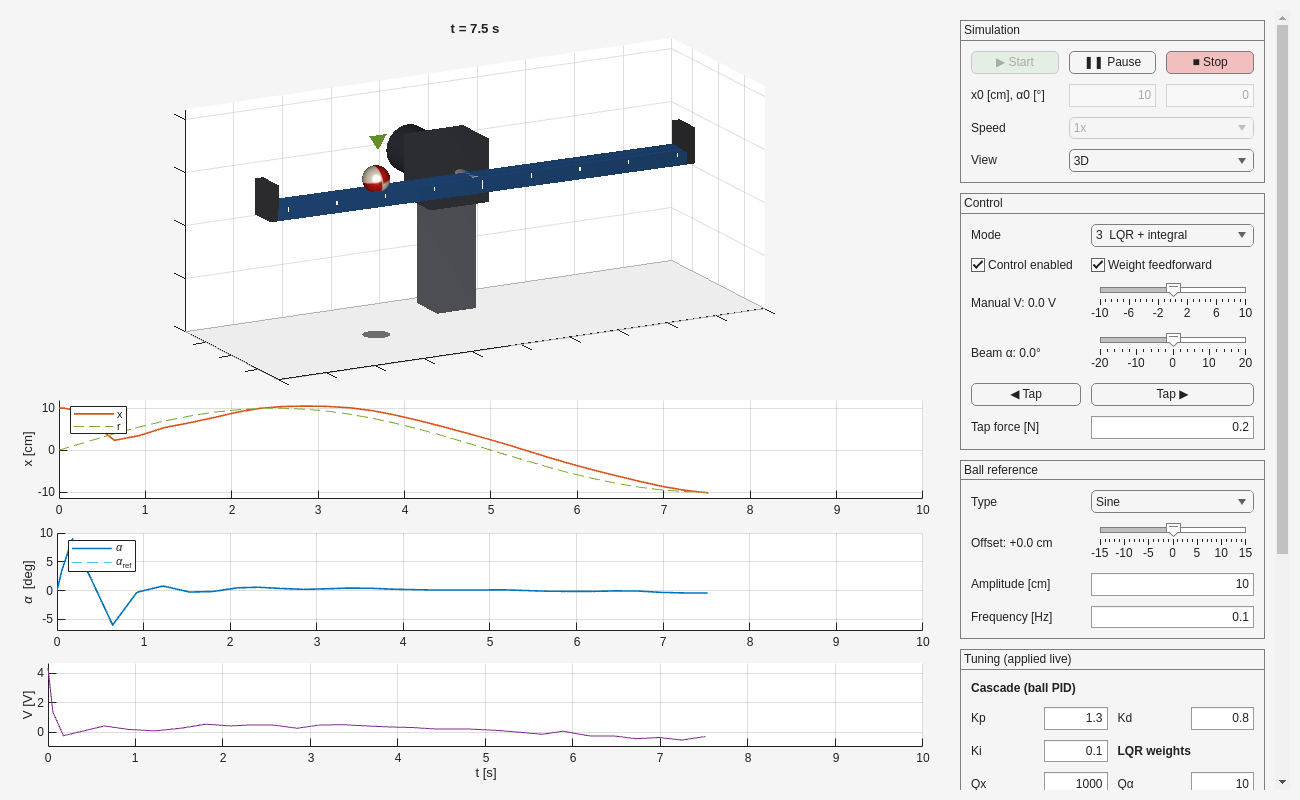
\includegraphics[width=\linewidth]{data/gui.png}
\caption{La GUI siguiendo en vivo una referencia senoidal de $\pm\SI{10}{cm}$ a \SI{0.1}{Hz} con el LQR.}
\label{fig:gui}
\end{figure}

\paragraph{La escena 3D.} La dibuja \code{bb\_draw}: la base, el pedestal, el motor con su reductora detrás de la viga, la viga (con una escala en centímetros y los topes de los extremos), la bola y su sombra. La bola tiene dos colores para que se vea rodar. El triángulo verde marca la referencia $r$. Se puede girar con el ratón o elegir otro punto de vista en la lista \textbf{View} (3D, \emph{Front}, \emph{Top}, \emph{Side}); desde código, con \code{bb\_view(ax, nombre)}.

\paragraph{Uso típico.}
\begin{enumerate}
  \item Elegir la posición inicial de la bola (cm) y el ángulo inicial de la viga ($^\circ$), y la velocidad de simulación.
  \item Pulsar \textbf{Start}. Desde ese momento, cualquier cambio de modo, referencia, tensión, ganancias de la cascada o pesos del LQR se aplica en vivo.
  \item Con la ventana activa, las teclas $\leftarrow/\rightarrow$ dan un golpecito a la bola hacia $-x$/$+x$ y, en el modo \code{beam}, $\uparrow/\downarrow$ cambian el ángulo de la viga en $\pm1^\circ$.
  \item La casilla \emph{Weight feedforward} activa o desactiva la compensación del peso de la bola (sección~\ref{sec:ff}).
  \item \textbf{Stop} y después \textbf{Export last run}: los datos quedan en \code{bb\_res} y se representan con \code{bb\_plot\_results}.
\end{enumerate}

\chapter{Prácticas guiadas}
\label{cap:practicas}

Las prácticas están ordenadas de menor a mayor dificultad y siguen el mismo esquema que las de los péndulos: objetivos, procedimiento con el código necesario, cuestiones y entregables. Al empezar cada sesión conviene ejecutar:
\begin{lstlisting}
clear; close all; bb = BallBeam(); bb.clearSignals();
\end{lstlisting}
Los valores que se citan como referencia corresponden a los parámetros por defecto. Recuerda que la interfaz de código trabaja en metros y radianes.

% ----------------------------------------------------------------
\refstepcounter{practica}\label{pr:explora}
\begin{practica}{Exploración y validación del modelo}
\objetivos
\begin{itemize}
  \item Familiarizarse con la interfaz y la animación 3D.
  \item Comprobar el factor $\tfrac57$ de la rodadura y el polo inestable del modelo lineal.
\end{itemize}
\procedimiento
\begin{enumerate}
  \item Inclinar la viga con el servo del modo \code{beam} y dejar rodar la bola:
\begin{lstlisting}
bb.setMode('beam'); bb.setInitialState([0 0 0 0]);
for a = [-1 -2 -4]
    bb.setBeamAngle(deg2rad(a)); res = bb.run(3);
    plot(res.t, res.x_cm); hold on
end
\end{lstlisting}
  Ajustar $x(t)=\tfrac12at^2$ al primer tramo y comparar $a$ con $\tfrac57g\sin\alpha$.
  \item Repetir con una bola hueca: en \code{bb\_derived.m} cambiar $J_b$ a $\tfrac23mr_b^2$ y volver a crear el objeto. ¿Qué factor se obtiene ahora?
  \item Con el modo \code{open}, la bola en $x_0=\SI{2}{cm}$ y $V=0$, observar cómo cae la viga hacia el lado de la bola. Ajustar una exponencial a los primeros instantes y compararla con el polo $+3{,}62$ (tabla del capítulo~\ref{cap:analisis}).
\end{enumerate}
\preguntas
\begin{enumerate}
  \item ¿Por qué el factor $\tfrac57$ no depende ni de la masa ni del radio de la bola?
  \item ¿Por qué el tiempo hasta el tope es algo mayor que la predicción con la viga fija? (Pista: mirar $\alpha(t)$.)
  \item Explicar con~\eqref{eq:caract} de dónde sale el polo inestable si la ecuación de la bola sola es un doble integrador.
\end{enumerate}
\entregables Gráficas de los ensayos y tabla comparativa entre teoría y simulación.
\end{practica}

% ----------------------------------------------------------------
\refstepcounter{practica}\label{pr:interno}
\begin{practica}{Diseño del lazo interno}
\objetivos Ajustar el servo de posición de la viga y entender por qué debe ser rápido y rígido.
\procedimiento
\begin{enumerate}
  \item Retirar la bola (\code{bb.setParam('m', 1e-5)}) y aplicar escalones de $5^\circ$ en modo \code{beam} (figura~\ref{fig:interno}).
  \item Calcular $K_{pa}$ y $K_{da}$ para $\omega_n\in\{15,\ 27,\ 50\}$~rad/s con $\zeta=0{,}7$ a partir de $Js^2+(b_{\text{eq}}+k_vK_{da})s+k_vK_{pa}$ y comprobarlos (\code{bb.setParams(struct('Kp\_a', ..., 'Kd\_a', ...))}).
  \item Volver a poner la bola en $x=\SI{15}{cm}$ con la viga horizontal y medir cuánto se inclina la viga en los primeros \SI{0.2}{s} con cada ajuste.
  \item Medir el error en régimen permanente del escalón y relacionarlo con la fricción de Coulomb $T_c$.
\end{enumerate}
\preguntas
\begin{enumerate}
  \item ¿Qué limita la rapidez del lazo interno: la tensión, el ruido del encoder o el periodo de muestreo?
  \item ¿Qué rigidez angular (N\,m/rad) tiene la viga con el PD por defecto? ¿Cuánto la inclina la bola en el extremo?
\end{enumerate}
\entregables Tabla de ajustes con $\omega_n$, $\zeta$, sobreoscilación, $t_{95}$ y error permanente.
\end{practica}

% ----------------------------------------------------------------
\refstepcounter{practica}\label{pr:cascada}
\begin{practica}{Control en cascada y prealimentación}
\objetivos Diseñar el lazo externo sobre la planta simplificada $-\tfrac57g/s^2$ y verificar la importancia de compensar el peso.
\procedimiento
\begin{enumerate}
  \item Elegir $K_{px}$ y $K_{dx}$ para un lazo externo con $\omega_n\in\{2,\ 3,\ 5\}$~rad/s y $\zeta=0{,}9$. Probar cada diseño con un escalón de \SI{10}{cm} en modo \code{cascade}.
  \item Encontrar a partir de qué $\omega_n$ del lazo externo la cascada empieza a oscilar. Relacionarlo con la $\omega_n$ del lazo interno.
  \item Con $K_{ix}=0$, desactivar la prealimentación (\code{ff\_on = 0}) y medir el error permanente para $r\in\{5,10,15\}$~cm. Compararlo con la predicción de la sección~\ref{sec:ff}.
  \item Activar de nuevo el integrador sin prealimentación. ¿Cuánto tarda en corregir el error? Probar $e_{\text{int}}=\SI{20}{cm}$ (integrador siempre activo) y observar la sobreoscilación por \emph{windup}.
\end{enumerate}
\preguntas
\begin{enumerate}
  \item ¿Qué regla práctica de separación entre los lazos interno y externo deducís?
  \item ¿Por qué la prealimentación usa la $x$ medida en la cascada y la referencia $r$ en el LQR?
\end{enumerate}
\entregables Diseños, respuestas al escalón y tabla de errores permanentes.
\end{practica}

% ----------------------------------------------------------------
\refstepcounter{practica}\label{pr:lqr}
\begin{practica}{Diseño de un LQR con acción integral}
\objetivos Entender el compromiso entre rapidez, inclinación de la viga y esfuerzo, y comparar con la cascada.
\procedimiento
\begin{enumerate}
  \item Desde $x_0=\SI{10}{cm}$, repetir el ensayo con $Q_x\in\{200,1000,5000\}$ y $R\in\{0{,}1,\ 1,\ 10\}$ (figura~\ref{fig:pesos}).
  \item Aplicar la regla de Bryson con $x_{\max}=\SI{2}{cm}$, $\alpha_{\max}=10^\circ$ y $V_{\max}=\SI{5}{V}$. Comparar con el diseño por defecto.
  \item Barrer $Q_\xi\in\{20,200,2000\}$ y medir a la vez la sobreoscilación del escalón y el tiempo de recuperación tras un golpecito de \SI{0.2}{N}$\times$\SI{50}{ms}.
  \item Comparar el mejor LQR con la mejor cascada de la práctica anterior en las tres pruebas: escalón, golpecito y senoide de \SI{0.25}{Hz}.
\end{enumerate}
\preguntas
\begin{enumerate}
  \item ¿Por qué el diseño con $R=0{,}1$ es más lento que el de $R=1$?
  \item ¿Qué peso controla la inclinación máxima de la viga? ¿Se podría añadir una restricción explícita?
\end{enumerate}
\entregables Tabla de diseños con sus métricas y una recomendación justificada.
\end{practica}

% ----------------------------------------------------------------
\refstepcounter{practica}\label{pr:segui}
\begin{practica}{Seguimiento de trayectorias}
\objetivos Medir el ancho de banda del lazo cerrado y mejorarlo con una prealimentación de la referencia.
\procedimiento
\begin{enumerate}
  \item Referencias senoidales de $\pm\SI{10}{cm}$ a 0,1; 0,25; 0,5 y \SI{1}{Hz} con ambos controladores. Medir ganancia y desfase (tabla~\ref{tab:sine}) y dibujar el Bode del lazo cerrado.
  \item Para que la bola siga $r(t)$ hace falta una inclinación $\alpha_{\text{ff}}=-\tfrac75\ddot r/g$. Añadirla a $\alpha_r$ en la cascada como modo 4 (sección~\ref{sec:nuevo_modo}), con $\ddot r$ calculada analíticamente para la senoide.
  \item Repetir las senoides con el modo nuevo.
  \item Probar una referencia triangular y una cuadrada. ¿Qué ocurre con la prealimentación en las esquinas?
\end{enumerate}
\preguntas
\begin{enumerate}
  \item ¿Hasta qué frecuencia se puede seguir una senoide de \SI{10}{cm} sin llegar a los topes de la viga? (Calcular la inclinación necesaria.)
  \item ¿Por qué el limitador de pendiente de la referencia mejora los escalones pero empeora las senoides rápidas?
\end{enumerate}
\entregables Bode del lazo cerrado con y sin prealimentación de la referencia.
\end{practica}

% ----------------------------------------------------------------
\refstepcounter{practica}\label{pr:robustez}
\begin{practica}{Robustez}
\objetivos Evaluar la sensibilidad de ambos controladores a errores de modelo.
\procedimiento
\begin{enumerate}
  \item Reproducir la tabla~\ref{tab:masa}. Repetirla con la prealimentación calculada con la masa \emph{nominal}. Como la planta y el controlador leen la misma \code{P.m}, hay que añadir un parámetro \code{m\_ff} y usarlo en \code{bb\_controller\_block.m}.
  \item Multiplicar la fricción de Coulomb de la viga por 5 (\code{setParamRaw('Tc', 0.05)}) y observar los ciclos límite de la bola con y sin integrador.
  \item Cambiar la longitud de la viga (\code{setParam('L', 0.6)}) sin recalcular las ganancias del LQR.
\end{enumerate}
\preguntas ¿Qué controlador es más robusto frente a cada error de modelo? Relacionar las respuestas con la estructura de cada uno.
\entregables Tabla de robustez y una discusión de una página.
\end{practica}

% ----------------------------------------------------------------
\refstepcounter{practica}\label{pr:obs}
\begin{practica}{Instrumentación y observador de estado}
\objetivos Cuantificar el efecto del ruido y sustituir las derivadas filtradas por un observador.
\procedimiento
\begin{enumerate}
  \item Con el ruido activado, barrer $\tau_x\in\{5,10,20,50\}$~ms y representar el rizado de $V$ frente al tiempo de asentamiento.
  \item Diseñar un filtro de Kalman estacionario discreto para el modelo lineal, con las varianzas de medida $\sigma^2+q^2/12$ de cada sensor. Implementarlo como modo 5 en \code{bb\_controller\_block.m} con \code{persistent shat}.
  \item Comparar el modo 5 con el modo 3 en rizado de tensión, error de posición y respuesta al golpecito.
  \item Construir un observador que use \emph{solo} el encoder de la viga (el sistema es observable desde $\alpha$, capítulo~\ref{cap:analisis}) y comprobar lo mal condicionado que está.
\end{enumerate}
\preguntas ¿Merece la pena una pista resistiva de más resolución, o es mejor filtrar? ¿Qué pasaría con una cámara a \SI{30}{fps} en lugar de la pista? (Véase el manual de la bola y plato~\cite{placa}.)
\entregables Código del modo nuevo y comparación cuantitativa.
\end{practica}


\appendix
\chapter{Tabla de parámetros}
\label{cap:parametros}

\begin{table}[H]
\centering\footnotesize
\begin{tabularx}{\linewidth}{@{}p{4.1cm}p{3.6cm}p{2.1cm}X@{}}
\toprule
Campo de \code{P} & Valor & Unidad & Descripción\\
\midrule
\multicolumn{4}{@{}l}{\textit{Bola y viga}}\\
\code{m}, \code{rb}, \code{bx} & 0,067 / 0,0127 / $2\cdot10^{-3}$ & kg, m, N\,s/m & bola maciza de acero\\
\code{L}, \code{mbeam} & 0,42 / 0,35 & m, kg & viga\\
\code{Db}, \code{Tc}, \code{w\_eps} & $10^{-3}$ / 0,01 / 0,05 & N\,m\,s/rad, N\,m, rad/s & fricción de la viga\\
\code{Jb}, \code{mb}, \code{J}, \code{x\_max}, \code{kv}, \code{beq} & derivados (\code{bb\_derived}) & -- & capítulo~\ref{cap:modelo}\\
\multicolumn{4}{@{}l}{\textit{Motor y topes}}\\
\code{Rm}, \code{kt}, \code{km}, \code{Jm} & 2,6 / 0,00768 / 0,00768 / $3{,}9\cdot10^{-7}$ & $\Omega$, N\,m/A, V\,s/rad, kg\,m$^2$ & motor de continua\\
\code{Kg}, \code{eta\_g}, \code{eta\_m} & 70 / 0,9 / 0,69 & -- & reductora y rendimientos\\
\code{Vmax} & 10 & V & saturación del amplificador\\
\code{al\_max}, \code{k\_al}, \code{c\_al} & 0,35 / 200 / 2 & rad, N\,m/rad, N\,m\,s/rad & topes de la viga\\
\code{k\_x}, \code{c\_x} & 2000 / 5 & N/m, N\,s/m & topes de la bola\\
\multicolumn{4}{@{}l}{\textit{Sensores y tiempos}}\\
\code{res\_al}, \code{res\_x} & $2\pi/4096$ / $L/4096$ & rad, m & resolución de los sensores\\
\code{noise\_on}, \code{noise\_x}, \code{noise\_al} & 0 / $10^{-3}$ / $10^{-3}$ & --, m, rad & ruido de medida\\
\code{Ts}, \code{h} & 0,002 / 0,001 & s & muestreo y paso del solver\\
\code{tau\_v}, \code{tau\_x} & 0,005 / 0,02 & s & filtros derivativos (viga, bola)\\
\code{x0} & $[0{,}1;\ 0;\ 0;\ 0]$ & -- & estado inicial\\
\multicolumn{4}{@{}l}{\textit{Referencia y controladores}}\\
\code{x\_ref\_max}, \code{ref\_rate} & 0,15 / 0,3 & m, m/s & saturación y pendiente de la referencia\\
\code{Kp\_a}, \code{Kd\_a} & 40 / 1,5 & V/rad, V\,s/rad & PD de la viga (lazo interno)\\
\code{Kp\_x}, \code{Kd\_x}, \code{Ki\_x} & 1,3 / 0,8 / 0,1 & rad/m, rad\,s/m, rad/(m\,s) & PID de la bola (lazo externo)\\
\code{I\_max}, \code{e\_int}, \code{al\_ref\_max} & 0,5 / 0,02 / 0,25 & m\,s, m, rad & antisaturación y límite de $\alpha_r$\\
\code{ff\_on} & 1 & -- & prealimentación del peso de la bola\\
\code{Q}, \code{R} & diag(1000; 50; 10; 0,5; 200) / 1 & -- & LQR con integral\\
\code{K} & calculada (\code{bb\_design}) & -- & ganancia LQR\\
\bottomrule
\end{tabularx}
\caption{Parámetros por defecto (\code{bb\_params.m}).}
\end{table}

\chapter{Validación del modelo Simulink}
\label{cap:validacion}

Las gráficas de este manual se obtuvieron simulando \code{ballbeam\_sim.slx} (MATLAB R2025b, ode4, $h=\SI{1}{ms}$) con \code{data/generate\_data.m}. Para detectar errores de implementación, los mismos escenarios se ejecutaron también en una réplica independiente en Python (\code{python\_reference\_sim.py}) y se compararon muestra a muestra. La réplica no modela el limitador de pendiente de la referencia, así que en esta comparación se desactivó.

\begin{table}[H]
\centering\small
\begin{tabularx}{\linewidth}{@{}lrrX@{}}
\toprule
Escenario & RMS $\Delta x$ [mm] & RMS $\Delta\alpha$ [$^\circ$] & Métrica (Python / Simulink)\\
\midrule
LQR desde $x_0=\SI{10}{cm}$ & 0,060 & 0,018 & asentamiento a \SI{5}{mm}: 0,68 / 0,68 s; $V_{\max}$ 4,3 / 4,3 V\\
LQR, escalón \SI{10}{cm} & 0,056 & 0,016 & asentamiento 0,64 / 0,64 s; sobreoscilación 2,5 / 2,5\,\%\\
LQR, golpecito & 0,110 & 0,026 & $\max|x|$ 1,89 / 1,93 cm\\
Cascada desde $x_0=\SI{10}{cm}$ & 0,043 & 0,013 & asentamiento 1,52 / 1,52 s; $V_{\max}$ 5,7 / 5,7 V\\
Cascada, escalón \SI{10}{cm} & 0,039 & 0,012 & asentamiento 1,50 / 1,50 s; final 10,07 / 10,07 cm\\
Cascada, golpecito & 0,108 & 0,024 & $\max|x|$ 1,66 / 1,69 cm\\
Cascada sin prealimentación & 0,041 & 0,012 & final 11,07 / 11,07 cm\\
Viga a $-2^\circ$, bola libre & 0,314 & 0,007 & llega al tope en 1,249 / 1,250 s\\
\bottomrule
\end{tabularx}
\caption{Comparación entre la réplica en Python y el modelo Simulink.}
\label{tab:validacion}
\end{table}

Las discrepancias son del orden de la resolución del sensor de posición (\SI{0.10}{mm}); la mayor aparece en el ensayo de la bola libre, en el que la bola se acelera sin control y cualquier diferencia de un paso de muestreo crece con el tiempo. Además se comprobó que una sesión en vivo (\code{start}/\code{stop}, también lanzada desde la GUI) reproduce la misma trayectoria que \code{run}.

Para repetir la validación:
\begin{lstlisting}
cd src/ball_beam/validation
run_validation                         % MATLAB: escribe results/*.csv
!python3 compare_with_python.py        % compara con la réplica en Python
\end{lstlisting}

\chapter{Resolución de problemas}

\begin{table}[H]
\centering\small
\begin{tabularx}{\linewidth}{@{}p{4.8cm}X@{}}
\toprule
Síntoma & Solución\\
\midrule
\emph{Undefined variable P} al pulsar \emph{Run} en Simulink & Ejecutar \code{BallBeam()} o \code{P = bb\_design(bb\_params())}. La \code{InitFcn} lo hace sola si el modelo se ha generado con el script.\\
Los cambios en \code{bb\_*\_block.m} no tienen efecto & Volver a ejecutar \code{bb\_build\_model}: el código se copia dentro del modelo al generarlo.\\
\code{setParamRaw('m', \ldots)} no cambia las inercias & Las magnitudes derivadas solo se recalculan con \code{setParam}. Para mantener las ganancias nominales, imponerlas después con \code{setParamRaw('K', K)}.\\
La bola se queda a \SI{1}{cm} de la referencia & La prealimentación del peso está desactivada (\code{ff\_on = 0}) y el integrador apagado ($K_{ix}=0$) o fuera de su banda.\\
La bola oscila alrededor de la referencia con amplitud pequeña & Fricción de Coulomb de la viga más cuantización: subir $K_{pa}$ o activar el integrador.\\
La viga golpea los topes & Pesos del LQR demasiado agresivos o referencia sin limitador: reducir $Q_x$ o \code{x\_ref\_max}.\\
La animación va a saltos & La clase reduce la frecuencia de la telemetría si la GUI no da abasto (\code{GuiLoad}). La simulación no se ve afectada: solo se pierden fotogramas.\\
\bottomrule
\end{tabularx}
\caption{Problemas habituales.}
\end{table}


\begin{thebibliography}{9}
\bibitem{hauser1992} J.~Hauser, S.~Sastry y P.~Kokotović, «Nonlinear control via approximate input-output linearization: the ball and beam example», \emph{IEEE Transactions on Automatic Control}, 37(3):392--398, 1992.
\bibitem{astrom} K.~J.~Åström y R.~M.~Murray, \emph{Feedback Systems: An Introduction for Scientists and Engineers}, 2.ª ed., Princeton University Press, 2021.
\bibitem{lineal} \emph{Péndulo lineal (carro-péndulo): manual teórico y práctico}, primer experimento de esta serie (\code{doc/linear\_pendulum\_manual.pdf}).
\bibitem{rotacional} \emph{Péndulo rotacional (péndulo de Furuta): manual teórico y práctico}, segundo experimento de esta serie (\code{doc/rotary\_pendulum\_manual.pdf}).
\bibitem{placa} \emph{Bola y plato: manual teórico y práctico}, cuarto experimento de esta serie (\code{doc/ball\_plate\_manual.pdf}).
\end{thebibliography}

\end{document}
